\documentclass[12pt]{article}
%\usepackage{proceed2e}
\usepackage{amsmath, amsthm, amssymb}
\usepackage{graphicx}
\usepackage{color}
\usepackage{xcolor}
\usepackage{listings}
\usepackage{inconsolata}
\usepackage[numbers]{natbib}
\usepackage{hyperref}
\usepackage{colonequals}
\usepackage{todonotes}
%\usepackage{bm}
\usepackage{gb4e}
%\usepackage{MnSymbol}
%\usepackage{stmaryrd}
%\usepackage{amsfonts}
\usepackage[small]{caption}

\newcommand{\llbracket}{\ensuremath{\left [\!\left [}}%
\newcommand{\rrbracket}{\ensuremath{\right ]\!\right ]}}
\providecommand{\sv}[1]{\ensuremath{\llbracket #1 \rrbracket}}
\providecommand{\textsv}[1]{\ensuremath{\llbracket \text{#1} \rrbracket}}
%\newcommand{\lar}[1]{\ensuremath{\langle #1 \rangle}}
\newcommand{\denot}[1]{\ensuremath{\llbracket \mathit{#1} \rrbracket}}

\newenvironment{AY11-12}{}{}

%\usepackage[raggedright]{sidecap}
%\usepackage{multirow}

 
 
 \lstset{
  language=Scheme, % Andreas Stuhlmüller. Scheme listings. https://github.com/stuhlmueller/scheme-listings.git
  columns=fixed,
  keepspaces,
  tabsize=2,
  extendedchars=true,
  breaklines=true,
  frame=single,
  numbers=left,
  numbersep=5pt,
  rulesepcolor=\color{solarized@base03},
  numberstyle=\tiny\color{solarized@base01},
  basicstyle=\scriptsize\ttfamily,
  keywordstyle=\color{solarized@green},
  stringstyle=\color{solarized@cyan}\ttfamily,
  identifierstyle=\color{solarized@blue},
  commentstyle=\color{solarized@base01},
  emphstyle=\color{solarized@red}
}

\definecolor{solarized@base03}{HTML}{002B36}
\definecolor{solarized@base02}{HTML}{073642}
\definecolor{solarized@base01}{HTML}{586e75}
\definecolor{solarized@base00}{HTML}{657b83}
\definecolor{solarized@base0}{HTML}{839496}
\definecolor{solarized@base1}{HTML}{93a1a1}
\definecolor{solarized@base2}{HTML}{EEE8D5}
\definecolor{solarized@base3}{HTML}{FDF6E3}
\definecolor{solarized@yellow}{HTML}{B58900}
\definecolor{solarized@orange}{HTML}{CB4B16}
\definecolor{solarized@red}{HTML}{DC322F}
\definecolor{solarized@magenta}{HTML}{D33682}
\definecolor{solarized@violet}{HTML}{6C71C4}
\definecolor{solarized@blue}{HTML}{268BD2}
\definecolor{solarized@cyan}{HTML}{2AA198}
\definecolor{solarized@green}{HTML}{859900}

\oddsidemargin 0.0in 
%%this makes the odd side margin go to the default of 1inch
\textwidth 6.5in
%%sets the textwidth to 6.5, which leaves 1 for the remaining right margin with 8 1/2X11inch paper 

%\pagestyle{empty}
 

\newcommand{\theory}{...ToW theory...}


\title{Uncertainty in Language and Thought}


\begin{document}

\listoftodos
\pagebreak


\maketitle

\abstract{}




\tableofcontents

\pagebreak



Words are used to communicate ideas. Ideas are mental tools for coping with a complex and uncertain world. This implies that human conceptual structures should be key to word meaning, and that probability, the mathematics of uncertainty, should be indispensable for describing both language and thought. Indeed, probabilistic models have proven enormously useful in modeling human cognition \cite{Tenenbaum, etc}, and aspects of natural language \cite{ChaterManning}. Natural language semantics and pragmatics have only recently been attacked with probabilistic tools. In this chapter we synthesize several of these modeling advances, exploring a formal model of semantics grounded, via pragmatic inference, in core conceptual structures.



%\todo[inline]{Noah: This intro (taken from the lexsem grant) needs to be edited into something short and to the point...}
%
%Words are potentially one of the clearest windows on human knowledge and conceptual structure. 
%If we understood the connection between words and mental representation, we could gain critical insights into almost every aspect of psychology, construct vastly more useful thinking machines, and interface the two. 
%But what do words mean? In this project we aim to {\bf construct and explore a formal model of lexical semantics grounded, via pragmatic inference, in core conceptual structures}. 
%We will do so using a set of modeling tools---chiefly the probabilistic programming language Church \cite{goodman2008}---that we have previously developed and used to explain  aspects of high-level human cognition.

Flexible human cognition is derived in large part from our ability to imagine possible worlds (or situations). 
A rich set of concepts, intuitive theories, and other mental representations support imagining and reasoning about possible worlds---together we call these the conceptual lexicon. 
%
We can formalize the conceptual lexicon using probabilistic programming tools, viewing commonsense knowledge as a set of interrelated definitions (or concepts) in a probabilistic programming language. 
Probabilistic programs specify sampling procedures over possible program executions, each execution fixes (some of) the variables that describe the world, hence each collection of concepts describes how to sample from a rich space of possible worlds. 
The inference (or conditioning, or query) operator describes how to use these distributions on worlds for reasoning. 
%
We have been able to explain many inferences that humans draw from sparse evidence using these tools. 
Here we posit that this collection of concepts also forms the set of primitive elements available for lexical semantics: word meanings can be built from the pieces of conceptual structure.

However, the connection between core concepts and lexical semantics is not direct: 
first, because language must flexibly adapt to the context of communication, the connection between lexical representation and interpreted meaning is mediated by pragmatic inference;
second, sentence meanings act as constraints on possible worlds, via their truth-value, whereas core concepts describe generation of possible worlds.
We propose to explore a model of language that formalizes and explains these differences, again using tools of probabilistic programming. 

In recent work we have made preliminary progress at combining underspecified semantic representations with a general purpose pragmatic inference mechanism.
This potentially allows us to account for subtle aspects of language use with relatively simple semantic denotations.
%: aspects of conveyed meaning emerge from an interaction of semantic denotation with context and core conceptual structures.
In particular, we view semantic representation as indivisible from core cognition, and the effective meaning of words as emerging from a pragmatic inference process. 

Our approach is similar in spirit to cognitive semantics, in that we attempt to ground semantics in mental representation, but we draw on the highly successful tools of Bayesian cognitive science to formalize these ideas. 
Similarly, our approach draws heavily on the progress made in formal model-theoretic semantics \cite{montague1973,heimkratzer1998}, borrowing insights about how syntax drives semantic composition, but we compose elements of stochastic logics rather than deterministic ones.
%Finally, our approach is related to recent progress in robotics (and indeed our project will benefit from ongoing collaboration with roboticist Stefanie Tellex of Brown University), but is more systematic and systematically connected to cognitive and linguistic theory. 

%We propose to study lexical semantics in the setting of an architecture for language understanding that is described in section \ref{langaugemodels}. 
%We first provide, in section \ref{background}, background on the probabilistic programming language Church and on using Church to describe core cognition. 
%In section \ref{lex} we describe the case studies of lexical semantics that we propose to explore in this project. 
%We will rely heavily on computational infrastructure for inference in the Church language; the models we propose push the envelope of what is currently possible and will require new inference techniques. 
%In section \ref{infrastr} we describe proposed work on Church inference algorithms and implementations.
%
%Probabilities describe degrees of belief, and probabilistic inference describes rational reasoning under uncertainty. 
%It is no wonder, then, that probabilistic models have exploded onto the scene of modern artificial intelligence, cognitive science, and applied statistics: these are all sciences of inference under uncertainty. 
%But as probabilistic models have become more sophisticated, the tools to formally describe them and to perform probabilistic inference have wrestled with new complexity. 
%Just as programming more than the simplest algorithms requires tools for abstraction and composition, complex probabilistic modeling requires new progress in model representation---\emph{probabilistic} programming languages. 
%These languages provide compositional means for describing complex probability distributions; implementations of these languages provide \emph{generic} inference engines: tools for performing efficient probabilistic inference over an arbitrary program. 

%By providing a uniform and universal representation for probabilistic models, probabilistic programming provides a framework for unifying disparate Bayesian models of human cognition. 
%Indeed, while Bayesian models have been extremely influential in cognitive science \cite[e.g.][]{tenenbaum2011}, 
%it is only recently that we have the tools to view the Bayesian approach as a general framework for mental representation.
%We next give a brief introduction to probabilistic programming, then an indication of how these tools can be used for modeling human cognition.

%make sure to have something like this:
In this chapter we illustrate the use of probabilistic techniques in natural language pragmatics and semantics with a concrete formal model. This model is not meant to exhaust the space of possible probabilistic models, indeed dozens of extensions are immediately apparent, but rather to show that a probabilistic framework for natural language is possible and productive.



\section{Bayesian models of commonsense reasoning}
%\begin{itemize}

%\item  Knowledge as generative model, 
  
%\item  Conditioning. Reasoning as conditional inference. Observations. Sequences of observations are sequences of conditioning. More general conditions.
  
%\item  Stochastic lambda calculus. Compositional sampling semantics. Universality. 
%\subitem ESLC: xrps, query. mem or do random worlds variation?
%\subitem possible worlds, partial worlds, and the minimal-situation property of eval/query.
  
%\item Example: tug-of-war domain. Elaborated model with 'match' events that have teams and winners, 'team' entities that have players and captains, 'player's that have strengths and genders. show elaborated strength models that depends on players gender in an unknown way (i.e. simple mixture model)...  
  
%\item Basic effects: Explaining away + screening off. 
%\subitem  Observe sam beats jim, infer sam is stong. learn that jim is weak, explain away match outcome, so sam is ordinary strength again.
%\subitem  Observe sam beats jim, predict sam will beat jim again. Knowing jim and sam's strengths, finding out sam beat jim doesn't change prediction. 
%\subitem   Mention but don't illustrate other effects ---  Size principle / occam, transfer learning.
%  
%\item  Modularity vs joint inference: knowledge is modular, inference is not.
  
%\end{itemize}
 

Uncertainty is a key property of the world we live in, thus we should expect reasoning with uncertainty to be a key operation of our cognition. 
At the same time our world is built from a complex web of causal and other structures, so we expect structure within our representations of uncertainty. 
Structured knowledge of an uncertain world can be naturally captured by \emph{generative} models, which make it possible to flexibly imagine (simulate) possible worlds or situations in proportion to their likelihood. 
The tools of structured probabilistic modeling, and particularly the stochastic lambda calculus we will use in this chapter, allow us to formalize these notions. 
In this section, we first introduce the basic operations for dealing with uncertainty---degrees of belief and probabilistic conditioning. 
We then introduce formal tools for adding compositional structure to these models---the stochastic lambda calculus---and demonstrate how these tools let us build generative models of the world and capture commonsense reasoning. 
In later sections, we demonstrate how these tools can be used to provide new insights into issues in natural language semantics and pragmatics.

Probability is fundamentally a set of tools for manipulating degrees of belief. 
The probability\footnote{Everything we say here applies equally well to probability densities, and more generally probability measures, but we describe in terms of probabilities for simplicity.} of a proposition is simply a real number between $0$ and $1$ describing an agent's degree of belief in that proposition. 
More generally, a \emph{random variable} $A$ is an assignment of a probability $P(A{=}a)$ to each of a set of exhaustive and mutually exclusive outcomes $a$, such that $\sum_a P(A{=}a)=1$. 
The joint probability $P(A{=}a,B{=}b)$, of two random variable values) is the degree of belief we assign to the proposition that both $A{=}a$ and $B{=}b$. 

\todo[inline]{We should define ``distribution''  and ``marginal'' somewhere.} 

The fundamental operation for incorporating new information or assumptions $B$ into prior beliefs is \emph{probabilistic conditioning}. 
This operation takes us from the \emph{prior} probability of $A$, $P(A)$, to the \emph{posterior} probability of $A$ given $B$, written $P(A|B)$. 
Conditional probability is standardly defined, following \citet{kolmogorov33}, by:
\begin{equation}
\label{conditionaldef}
P(A|B) = \frac{P(A,B)}{P(B)} 
\end{equation}
This unassuming definition is the basis for much recent progress in modeling human reasoning \cite[e.g.][]{tenenbaum2011}: by modeling uncertain beliefs in probabilistic terms, we can understand reasoning as probabilistic conditioning. 
In particular, imagine a person who is trying to establish which hypothesis $H\in\{h_1,\dots,h_m\}$ best explains a situation, and does so on the basis of a series of observations $\{o_i\}_{i=1}^N$. 
We can describe this inference as the conditional probability:
\begin{equation}
P(H|o_1,\dots,o_N) = \frac{P(H)P(o_1,\dots,o_N|H)}{P(o_1,\dots,o_N)}.
\end{equation}
This useful equality is called \emph{Bayes' rule}; it follows immediately from the definition in equation \ref{conditionaldef}. 
If we additionally assume that the observations provide no information about each other beyond what they provide about the hypothesis, that is they are \emph{conditionally independent}, then $P(o_i|o_j, H)=P(o_i|H)$ for all $i\neq j$. 
It follows that:
\begin{equation}
P(H|o_1,\dots,o_N) = \frac{P(H)P(o_1|H)\cdots P(o_N|H)}{P(o_1|H)\cdots P(o_N|H)}.
\end{equation}
From this it is a simple calculation to verify that we can perform the conditioning operation sequentially rather than all at once: the \emph{a posteriori} degree of belief given observations $o_1,\dots,o_i$ becomes the \emph{a priori} degree of belief for incorporating observation $o_{i+1}$.
\todo[inline]{explain more, or put in as theorem? we want to call back to this in explaining the basic dynamic of belief updating from literal meaning...}
%Dan: Also, worth mentioning that the independence assumption isn't required to justify sequential conditioning as opposed to all-at-once.
%Noah: well independent given H is required...

\subsection{Stochastic Lambda Calculus and Church}

Probability as described so far provides a notation for indicating degrees of belief and conditional information, but requires that the actual probability distributions be specified separately (for example by writing down the numbers in a table); this quickly becomes unmanageable when we wish to describe complex knowledge---relations among many beliefs. 
The stochastic lambda calculus (SLC) provides a formal, compositional language for describing probabilities over complex sets of interrelated beliefs. 
We assume some familiarity with the (deterministic) lambda calculus \cite{lambda}. 
At its core SLC simply extends the lambda calculus with an expression type $(L \oplus R)$, indicating random choice between the sub-expressions $L$ and $R$, and an additional reduction rule that reduces such a choice expression to its left or right sub-expression with equal probability. 
While this reduction process results in a single expression after any sequence of reductions, it can be viewed as a distribution over such reduction sequences, and hence a distribution over the final expression: SLC expressions denote (sub-)distributions over completely reduced SLC expressions. 
It can be shown that this system can represent any computable distribution in an appropriate sense \cite[see for example][]{PfefferRamsey,FreeRoy}.

This simple calculus is universal but cumbersome to work with. 
\citet{Goodman2008} introduce Church, an enriched SLC that can be realized as a \emph{probabilistic programming language}, just as the programming language LISP is an enriched lambda calculus. 
Church starts with the pure subset of Scheme (which is itself essentially lambda calculus enriched with primitive data types, operators, and useful syntax) and extends it with elementary random primitives (ERPs), the inference function \lstinline{query}, and the memoization function \emph{mem}. 
We next describe key pieces of the language semantics; further details and examples of using Church for cognitive modeling can be found at \url{http://bit.ly/ProbMods}.
In what follows we will assume passing familiarity with the Polish notation used in LISP-family languages (fully parenthesized and operator initial), and will occasionally build on ideas from programming languages---\cite{SICP} is an excellent background on these ideas. 

Rather than restricting to the $\oplus$ uniform random choice between two options (which is sufficient, but results in extremely cumbersome representations), Church includes an interface for adding elementary random primitives (ERPs). These are procedures that return random values; a sequence of evaluations of such and ERP procedure is assumed to result in independent identically distributed (i.i.d.) values. Common ERPs include Bernoulli (\lstinline{flip}), \lstinline{uniform}, \lstinline{gaussian}, etc. While the ERPs themselves are i.i.d., it is straightforward to construct Church procedures sing ERPs that are not i.i.d. For instance:
\begin{lstlisting}[mathescape]
(define bias (uniform 0 1))
(define coin ($\lambda$ () (flip bias)))
\end{lstlisting}
Multiple calls to the function \lstinline{coin} will result in a sequence of values which are not i.i.d., because the jointly depend on the unknown \lstinline{bias} (though they are exchangeable \cite{defintetti}).

Memoization is a higher-order function that upgrades a stochastic function to have persistent randomness. 

mem

eval




\todo[inline]{Noah: give definitional interpreter (eval) for ESLC. need: define, xrps, query, mem.}


\label{bottom-val}
Church is a dynamically typed language: values have types, but expressions don't have fixed types that can be determined \emph{a priori}. For simplicity (and utility below) we assume that when an operator is applied to values outside of its domain, for instance \lstinline{(+ 1 'a)}, they return a special value \emph{error} which is itself outside the domain of all operators, except the equality operator \lstinline{eq?}. By allowing \lstinline{eq?} to test for error we permit very simple error handling.




\subsection{Commonsense knowledge}

A set of stochastic function definitions in Church can be interpreted as a distribution over possible worlds: A world consists of a value for each well-formed expression that can be made from the defined functions (in each calling position). 
To evaluate any particular expression or query requires evaluating only a small subset of this infinitude of expressions. 
That is, an particular query only depends on the partial world of expressions actually constructed during the evaluation process. 
The relationship between the idealized complete possible worlds and these partial worlds is coherent because taking the marginal sum over any expressions that are evaluated but that don't impact the value of the query (condition or query expressions) results in the same distribution as if we didn't evaluate them. 
\todo{Noah: need to state this theorem more formally.} 
For this reason we can comfortably speak interchangeably about possible worlds and partial worlds (or situations).

In this chapter we use sets of stochastic functions in Church to specify the intuitive knowledge---or theory---that a person has about the world. 
To make this more precise we now describe an example, the tug-of-war game, which we will use later in the chapter as the non-linguistic conceptual basis of a semantics and pragmatics for a small fragment of English. 
Tug-of-war is a simple game in which two teams pull on either side of a rope; the team that pulls hardest will win. 
Our intuitive knowledge of this domain (and indeed most similar team games) rests on a set of interrelated concepts: players, teams, strength, matches, winners, etc. 
We now sketch a simple realization of these concepts in Church. 
To start, each player has some traits that influence his or her contribution to the game: strength, which may depend on gender.
\begin{lstlisting}[mathescape]
(define gender (mem ($\lambda$ (p) (if (flip) `male `female))))
(define gender-mean-strength (mem ($\lambda$ (g) (gaussian 0 2))))
(define strength (mem ($\lambda$ (p) (gaussian (gender-mean-strength (gender p)) 1))))
\end{lstlisting}
We have defined the strength of a person as a \emph{mixture model}: strength depends on a latent class, gender, through the (a priori unknown) gender means. 
Note that we are able to describe the properties of people (\lstinline{strength}, \lstinline{gender}) without needing to specify the people---instead we assume that each person is represented by a unique symbol, and memoize the functions on this symbol, resulting in functions which create the properties of a person only when needed (but then hold those properties persistently). 
In particular, the person argument, \lstinline{p}, is never used in the function \lstinline{gender}, but it matters because the function is memoized---a gender will be persistently associated to each person though generating that gender initially doesn't depend on the person. 
We will exploit this pattern often below.
We are now already in a position to make useful inferences. 
We could, for instance observe the strengths and genders of several players, and then Pat's strength but not gender, and ask for the latter:
\begin{lstlisting}[mathescape]
(query
  (define gender (mem ($\lambda$ (p) (if (flip) `man `woman))))
  (define gender-mean-strength (mem ($\lambda$ (g) (gaussian 0 2))))
  (define strength (mem ($\lambda$ (p) (gaussian (gender-mean-strength (gender p)) 1))))
  
  (gender `Pat)
  
  (and (equal? (gender `Bob) `male) (= (strength `Bob) -1.1)
       (equal? (gender `Jane) `female) (= (strength `Jane) 0.5)
       (equal? (gender `Jim) `male) (= (strength `Jim) -0.3)
       (= (strength 'Pat) 0.7)))
\end{lstlisting}
\todo{run this simulation}
The result of this query is that Pat is female with probability XX---because the observed males are weaker than the observed female, Pat, who is strong, is likely female.

%\todo[inline]{We could already talk about explaining away and screening off here... should we?}
%\todo[inline]{I think it's more intuitive as you do it below, using results and inferring strengths.}
In the game of tug-of-war players are on teams, which themselves have properties such as captains:
\begin{lstlisting}[mathescape]
(define players `(Bob Jim Mary Sue Bill Evan Sally Tim Joe Jane Terrence Kate))
(define team-size (uniform-draw '(1 2 3 4 5 6)))
(define players-on-team (mem ($\lambda$ (team) (draw-n team-size players))))
(define captain (mem ($\lambda$ (team) (uniform-draw (players-on-team team)))))
\end{lstlisting}
Here the \lstinline{draw-n} ERP draws uniformly but without replacement from a list.
%
In addition to players and teams, we have matches: events that have two teams and a winner, the winner depends on how hard each team is pulling, which depends on how hard each team member is pulling.
\begin{lstlisting}[mathescape]
(define teams `(team1 team2 team3))

(define teams-in-match (mem ($\lambda$ (match) (draw-n 2 teams))))
(define pulling (mem ($\lambda$ (player match) (+ (strength player) (gaussian 0 0.5)))))
(define team-pulling (mem ($\lambda$ (team match) 
                                     (sum (map pulling (players-on-team team))))))
(define (winner match) 
  (let ([teamA (first (teams-in-match match))]
        [teamB (second (teams-in-match match))])
    (if (> (team-pulling teamA) (team-pulling teamB))
        teamA
        teamB)))
\end{lstlisting}
Notice that the team pulling is simply the sum of how hard each member is pulling; each player pulls with their intrinsic strength, plus a random amount that indicates their effort on this match. 
 
 \begin{figure}[tbh]
\begin{center}
 \begin{lstlisting}[mathescape]
(define players `(Bob Jim Mary Sue Bill Evan Sally Tim Joe Jane Terrence Kate))
(define teams `(team1 team2 team3))
(define matches `(match1 match2))

(define gender (mem ($\lambda$ (p) (if (flip) `male `female))))
(define gender-mean-strength (mem ($\lambda$ (g) (gaussian 0 2))))
(define strength (mem ($\lambda$ (p) (gaussian (gender-mean-strength (gender p)) 1))))

(define team-size (uniform-draw '(1 2 3 4 5 6)))
(define players-on-team (mem ($\lambda$ (team) (draw-n team-size players))))
(define captain (mem ($\lambda$ (team) (uniform-draw (players-on-team team)))))

(define teams-in-match (mem ($\lambda$ (match) (draw-n 2 teams))))
(define pulling (mem ($\lambda$ (player match) (+ (strength player) (gaussian 0 0.5)))))
(define team-pulling (mem ($\lambda$ (team match) 
                          (sum (map (lambda (x) (pulling x match)) (players-on-team team))))))
(define (winner match) 
  (let ([teamA (first (teams-in-match match))]
        [teamB (second (teams-in-match match))])
    (if (> (team-pulling teamA match) (team-pulling teamB match))
        teamA
        teamB)))
\end{lstlisting}
\caption{An intuitive theory (or conceptual lexicon) for the tug-of-war domain.}
\label{theory}
\end{center}
\end{figure}  

The conceptual lexicon of functions for the tug-of-war domain is given altogether in Figure \ref{theory}.
A conceptual lexicon like this one describes generative knowledge about the world---interrelated concepts that can be used to describe the causal story of how various observations come to be. 

We can use this knowledge to reason from observations to predictions or latent states by using conditionalization implemented via \lstinline{query}. 
Let us illustrate how a generative model is used to capture key patterns of reasoning. 
Imagine that Bob is playing Jim in match 1; we can infer Bob's strength before observing the outcome of this match:
\begin{lstlisting}[mathescape]
(query
  ...ToW theory...
  (strength `Bob) ;; variable of interest
  (and ;; conditioning expression 
    (equal? (players-on-team `team1) `(Bob))
    (equal? (players-on-team `team2) `(Jim))
    (equal? (teams-in-match `match1) `(team1 team2))))
\end{lstlisting}
In this and all that follows \lstinline{...ToW theory...} is an abbreviation for the definitions in figure \ref{theory}. 
The result of this strength is simply the prior belief about Bob's strength: a distribution with mean 0.0.

Now imagine that Bob wins this match:
\begin{lstlisting}[mathescape]
(query
  ...ToW theory...
  (strength `Bob) ;; variable of interest 
  (and ;; conditioning expression
    (equal? (players-on-team `team1) `(Bob))
    (equal? (players-on-team `team2) `(Jim))
    (equal? (teams-in-match `match1) `(team1 team2))
    (equal? (winner `match1) `team1)))
\end{lstlisting}
If we evaluate this query we find that Bob is inferred to be relatively strong: his mean strength after observing this match is about 1.2, much higher than his a priori mean strength of $0.0$). 
However, imagine that we then learned that Jim is a weak player:
 \begin{lstlisting}[mathescape]
(query
  ...ToW theory...
  (strength `Bob) ;; variable of interest 
  (and ;; conditioning expression
    (equal? (players-on-team `team1) `(Bob))
    (equal? (players-on-team `team2) `(Jim))
    (equal? (teams-in-match `match1) `(team1 team2))
    (equal? (winner `match1) `team1))
    (= (strength `Jim) -3.0))
\end{lstlisting}

Now, we have very little evidence about Bob's strength---the inferred mean strength from this query goes back to (almost) 0.0. 
This is an example of \emph{explaining away}: the assumption that Jim is weak has explained the observation that  Bob beat Jim, which otherwise would have provided evidence that Bob is strong. 
\begin{figure}[tbh]
\begin{center}
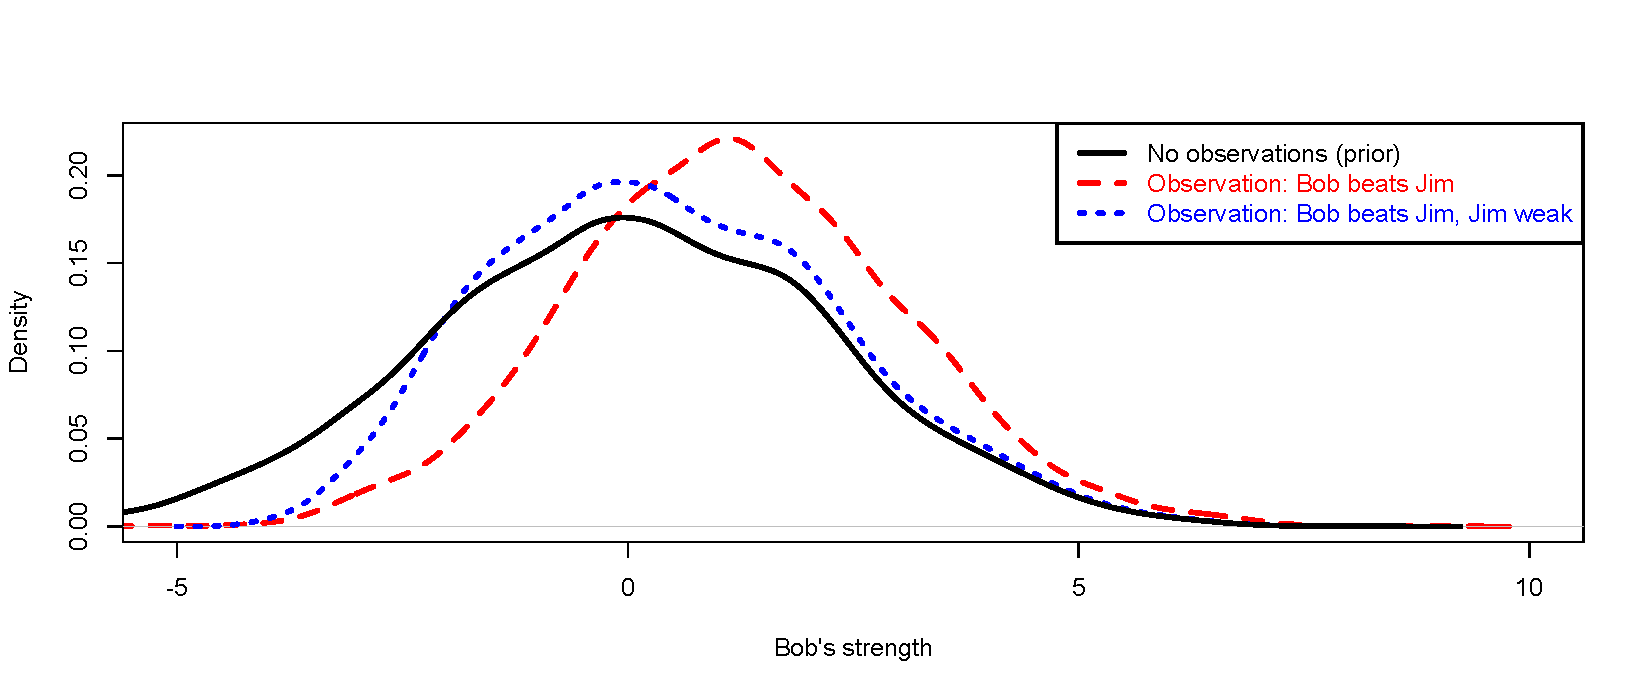
\includegraphics[scale=.65]{explaining-away-example.pdf}
\end{center}
\caption{An example of explaining away. 
Lines show the distribution on Bob's inferred strength after (a) no observations (solid); (b) observing that Bob beat Jim, whose strength is unknown (long dash); (c) learning that Jim is very weak, with strength -3 (short dash).}
\end{figure}
Notice that we have gone through a non-monotonic reasoning sequence: Our degree of belief that Bob is strong went up from the first piece of evidence, and then back down from the second. 
The explaining away pattern is extremely common in probabilistic inference over structure models. 
It is characterized by a priori independent variables (such as Bob and Jim's strengths) becoming coupled together by an observation (such as the outcome of match 1). 
Another way of saying this is that our knowledge of the world, the generative model, can have a significant amount of modularity; our inferences after making observations will generally not be modular in this way, instead complex patterns of influence can couple together disparate pieces of the model.

%Another common pattern is \emph{screening off}: 
% \todo[inline]{Observe sam beats jim, predict sam will beat jim again. Knowing jim and sam's strengths, finding out sam beat jim doesn't change prediction. }

There are a number of other patterns of reasoning that are common results of probabilistic inference over structured models. 
For instance, \emph{screening off} describes the situation when two variables that were a priori dependent become independent after an observation (in some sense the opposite of explaining away).
Other patterns include Occam's razor (complexity of hypotheses is automatically penalized), transfer learning (an inductive bias learned from one domain constrains interpretation of evidence in a new domain), and the blessing of abstraction (abstract knowledge can be learned faster than concrete knowledge). 
These will be less important in what follows, but we note that they are potentially important for the question of language learning---when we view learning as an inference, the dynamics of probabilistic inference come to bear on the learning problem. 
\todo{Citation for these and other patterns of inference}

 
\section{Meaning as condition}
\todo[inline]{Noah:
What if any general motivation do we give here?

Want to motivate meaning as conditioning from very general distributional assumptions. 
Sentences as observations. 
Assume sentences are independent (in literal meaning -- pragmatics changes this). 
Implies sentence composition by sequential conditioning.}

%This view of the belief states and their dynamics has a natural extension to language understanding: we can treat interpretation as conditioning on the literal meaning of a sentence. 

\subsection{\label{literal-listener}Literal interpretation}

Following a productive tradition in semantics and pragmatics \citep[][etc.]{stalnaker78,lewis79,heim82}, we view the basic function of language understanding as belief update: moving from a prior belief distribution over worlds (or situations) to a posterior belief distribution given the \emph{literal meaning} of a sentence. 
By analogy with the effects of observation on belief, we can formalize this idea naturally by defining the literal listener as:
\begin{lstlisting}
(define (literal-listener utterance QUD)
  (query
    ...theory...
    (eval QUD)
    (eval (meaning utterance))))
\end{lstlisting}
This function specifies the posterior distribution over answers to the Question Under Discussion (\lstinline{QUD}) given that the literal meaning of the utterance is true.\footnote{On QUD models, see \citealt{ginzburg95a,vankuppevelt95,roberts96,beaverclark08} among many others.} \todo{Noah: make sure the use of eval is clear.} Notice that the prior distribution is specified by a conceptual lexicon---the \lstinline{...theory...}. 

The \lstinline{meaning} function is a map from strings (surface forms) to Church expressions (logical forms, which include functions defined in \lstinline{...theory...}).
Many theories of syntactic and semantic composition could be used to provide this mapping. 
For concreteness, we consider a simple system in which a string is recursively split into left and right portions, and the meanings of these portions are combined with a random combinator:
\begin{lstlisting}
(define (meaning utterance)
  (if (lexical-item? utterance)
      (lexicon utterance)
      (let ([subs (random-split utterance)])
         ((random-combinator) (meaning (first subs)) (meaning (second subs))))))
\end{lstlisting}
Here the predicate \lstinline{lexical-item?} determines if the (remaining) utterance is a single lexical item (entry in the lexicon), if so it is looked up with the \lstinline{lexicon} function.
%\todo[inline]{``remaining'' suggests we're already within the recursion---maybe we should ease the poor linguists into it a bit?}
The function \lstinline{random-split} takes a string and returns the list of two substrings that result from splitting at a random position in the length of the string.
The function \lstinline{random-combinator} chooses a random composition operator, such as left application or right composition. 
We assume that the set of possible compositions is sufficient to perform any syntactic operations needed.\footnote{The set of composition operators includes at least forward and backward application and composition:
\begin{itemize}
\item \textbf{FA}: \lstinline{(lambda (A) (lambda (B) (A B)))}
\item \textbf{BA}: \lstinline{(lambda (A) (lambda (B) (B A)))}
\item \textbf{FC}: \lstinline{(lambda (A) (lambda (B) (lambda (x) (A (B x)))))}
\item \textbf{BC}: \lstinline{(lambda (A) (lambda (B) (lambda (x) (B (A x)))))}
\end{itemize}
We generate quantifier scope ambiguities by including among the set of composition operators all possible combinations of \textbf{FA}, \textbf{BA}, \textbf{FC}, and \textbf{BC} with the type-shifting mechanisms of \citet{hendriks93}. 
This treatment of quantifier scope is convenient, but others (e.g., quantifier raising or Skolem functions \cite{steedman12} ) could be implemented by complicating the syntactic or semantic mechanisms in various ways. 

Our simple implementation of \lstinline{random-split} does not insert silent elements such as indices and PRO. 
A complete theory would need to assume additional combinators to cope with gaps \citep{steedman00}, binding \citep{jacobson99,barker05}. 
Alternatively, it would a richer parsing mechanisms could create and interpret structures with silent elements and movement operations.}
Critically, if type errors are interpreted as the non-\emph{true} value \emph{error} (as described in section \ref{bottom-val}), then mis-typed compositions will not satisfy the condition of the \lstinline{query} in the \lstinline{literal-listener} function---though many ill-typed compositions can be generated by this procedure, they will be eliminated from the posterior, leaving only well-typed interpretations.
Thus the \lstinline{meaning} function is a stochastic mapping from strings to Church expressions; the random choices made in this mapping will be reasoned about jointly with world states while interpreting the utterance, as discussed in section \ref{ambiguity} below.

To understand what the \lstinline{literal-listener} does, consider rejection sampling: we evaluate both the \lstinline{QUD} and meaning expressions, constructing whatever intermediate expressions are required; if the meaning expression has value \lstinline{true}, then we return the value of \lstinline{QUD}, otherwise we try again. 
\todo[inline]{Dan: something about hyper intentionality? point out that the intention is a computation that can be run in a given intuitive theory environment. cite shalom ..}
It is apparent that the complexity of interpretation is an interaction between the domain theory, the meaning function, and the lexicon. 
To make this more concrete, we return to the tug-of-war example from the previous section and begin to build a lexicon for talking about this domain in natural language. 

\subsection{Interpreting English in Church: Lexicon and Composition}
\label{lexicon}
\todo[inline]{Noah: go through this section, clean up and move extra defs to a lexicon table.}
Natural language lexical items are interpreted as Church expressions, and sentence meanings are built up recursively from the denotations of lexical items along lines provided by the syntactic  structure. 
The \lstinline{lexicon} function maps English expressions to their interpretation in Church.
For simplicity we write the denotation \lstinline[mathescape]{(meaning $\cdot$)} as \denot{\cdot}. 

The stochastic $\lambda$-calculus (implemented in Church) thus functions as our intermediate translation language, just as the simply-typed $\lambda$-calculus functions as an intermediate translation language in Montague's \citeyear{montague73} fragment of English. 
A key difference, however, is that the intermediate level is not merely a convenience as in Montague's approach. 
Conceptual representations and world knowledge are also represented in this language (as Church function definitions)---use of a common language to represent linguistic and non-linguistic information makes it possible to model intricate interactions between these two types of knowledge. 

For example, the interpretation of a name is a Church symbol which is uniquely associated with some object or individual (the name-bearer). 
Interpreted in this way, names are directly referential since they are interpreted using the same symbol in every world, regardless of inferences made during interpretation. 
%does not depend on stochastic choices made in the interpretation process.
\begin{itemize}
\item \denot{Bob} = \lstinline{`Bob}
\item \denot{Team\ 1} = \lstinline{`team1}
\item \denot{Match\ 1} = \lstinline{`match1}
\item ...
\end{itemize}
A one-place predicate such as \emph{player} or \emph{man} is interpreted as a function from individuals to truth-values. 
Intensionality is implicit in these definitions, due to the fact that the denotations of English expressions can refer to stochastic functions in the intuitive theory, such as \lstinline{gender}.
\begin{itemize}
\item \sv{player} = \lstinline[mathescape]{($\lambda$ (x) (element? x player))}  
\item \sv{team} = \lstinline[mathescape]{($\lambda$ (x) (element? x teams))}
\item \sv{match} = \lstinline[mathescape]{($\lambda$ (x) (element? x matches))}
\item \sv{man} = \lstinline[mathescape]{($\lambda$ (x) (equal? (gender x) `male))}
\item \sv{woman} = \lstinline[mathescape]{($\lambda$ (x) (equal? (gender x) `female))}
\end{itemize}
Predicates denote intensions of properties: they pick out functions from individuals to truth-values in any world, but the specific function that they pick out in a world depends on the random choices (e.g., evaluations of \lstinline{flip}) that are made in the process of constructing the world. 
In these examples, \emph{player} is true of the same individuals in every world, since \lstinline{player} is defined deterministically in the intuitive theory in figure \ref{theory}. 
\emph{man}, on the other hand, denotes a predicate which will be true of a given individual (say, \lstinline{`Bob}) in 50\% of partial worlds constructed on average (assuming no relevant observations have been made). 
This is because the denotation of \emph{man} is a function which returns 1 if and only if its argument is an individual for which the \lstinline{gender} function returns \lstinline{`male}. 
\lstinline{gender}, in turn, is defined in figure \ref{theory} as a stochastic function which returns \lstinline{`male} and \lstinline{`female} with equal probability. 

Similarly, transitive verbs such as \emph{won} and relational nouns such as \emph{captain} denote the (stochastic) intensions of two-place predicates. 
(We simplify by ignoring tense.)
\begin{itemize}
\item \sv{won} = \lstinline[mathescape]{($\lambda$ (match) ($\lambda$ (x) (equal? x (winner match))))}
\item \sv{played\ in} =  \lstinline[mathescape]{($\lambda$ (match) ($\lambda$ (team-list) (all (map (lambda (x) (element? x (teams-in-match match)))) team-list)))} 
\item \sv{be\ on} =  \lstinline[mathescape]{($\lambda$ (team) ($\lambda$ (x) (element? x (players-on-team team))))} 
\item \sv{captain} = \lstinline[mathescape]{($\lambda$ (team) ($\lambda$ (x) (equal? x (captain team))))}
\end{itemize}
(We assume that the conjoined NP \emph{Team 1 and Team 2} denotes the list \lstinline{`(team1 team2)}; compare the set-based account of plurals described in Scha \& Winter, this volume.
Note that the denotation of \emph{played in} takes such a list as its second argument, but that the order of elements in the list does not matter.)


Gradable adjectives such as \emph{strong} and \emph{weak} denote relations between individuals and degrees \citep[][etc.]{cresswell76,vonstechow84}. 
The weakness scale is simply the strength scale with the sign reversed. 
\begin{itemize}
\item \sv{strong} = \lstinline[mathescape]{($\lambda$ (x) ($\lambda$ (d) (>= (strength x) d)))}
\item \lstinline{(define (weakness x) (- 0 (strength x))))}
\item \sv{weak} = \lstinline[mathescape]{($\lambda$ (x) ($\lambda$ (d) (>= (weakness x) d)))}
\end{itemize}
The interpretation of \emph{strong} and \emph{weak} as predicates requires pragmatic inference of the value of the vague threshold value: see section (\ref{vagueness}) below.

Finally, we define some functional vocabulary---a few quantificational determiners and the degree operator \emph{-est}---along with a domain of discourse relevant to the determiners.
\begin{itemize}
\item \lstinline{(define domain-of-individuals (union player team match))}
\item \sv{every} = \lstinline[mathescape]{($\lambda$ (P) ($\lambda$ (Q) (all (map ($\lambda$ (x) (not (and (P x) (not Q x)))) domain-of-individuals))))}
\item \sv{some} = \lstinline[mathescape]{($\lambda$ (P) ($\lambda$ (Q) (some (map ($\lambda$ (x) (and (P x) (Q x))) domain-of-individuals))))}
\item \sv{\text{-}est} = \lstinline[mathescape]{($\lambda$ (A) ($\lambda$ (N) ($\lambda$ (x) (= (argmax A x) (argmax ($\lambda$ (d) (some (map ($\lambda$ (x) (>= (A x) d)) N))))))))}
%\item \sv{the} = \lstinline[mathescape]{($\lambda$ (P) ($\lambda$ (x) (P x)))} 
\end{itemize}
The interpretations of \emph{every} and \emph{some} are standard. 
The superlative morpheme \emph{-est} is defined so that, for example, \emph{strongest player} will denote a property that is true of Bill if and only if the greatest degree of strength that Bill possesses is equal to the greatest degree of strength that any player possesses.

As an example of sequential interpretation by a literal listener, consider the output of the \lstinline{literal-listener} function in a variant of our explaining-away example from the previous section. 
Assume that the literal listener's initial belief state is as given in figure \ref{theory}, and his lexicon conforms to the definitions in this section. 
Then the literal listener will respond to the utterances below exactly as he would if he were to make observations which are encoded using the Church expressions by which the utterances are interpreted.\footnote{The interpretations below are examples of salient, simple interpretations that will be generated by the \lstinline{meaning} function as applied to these utterances; other interpretations may also be possible, depending on the parse generated by \lstinline{random-split} and the composition operators which \lstinline{random-combinator} chooses.}
\begin{itemize}
\item Utterance 1: ``Bob is on Team 1.''
\begin{itemize}
\item Possible interpretation: \textbf{BA}(\sv{Bob})(\textbf{FA}(\sv{be\ on})(\sv{Team\ 1}))
\item [$\equiv$] \sv{be\ on}(\sv{Team\ 1})(\sv{Bob})
\item [$=$] \lstinline[mathescape]{((($\lambda$ (team) ($\lambda$ (x) (element? x (players-on-team team)))) `team1) `Bob)}
\item [$\equiv$] \lstinline{(element? `Bob (players-on-team `team1))}
\end{itemize}
\item Utterance 2: ``Jim is on Team 2.''
\begin{itemize}
\item Possible interpretation: \textbf{BA}(\sv{Jim})(\textbf{FA}(\sv{be\ on})(\sv{Team\ 2}))
\item [$\equiv$] \sv{be\ on}(\sv{Team\ 2})(\sv{Jim})
\item [$=$] \lstinline[mathescape]{((($\lambda$ (team) ($\lambda$ (x) (element? x (players-on-team team)))) `team2) `Jim)}
\item [$\equiv$] \lstinline{(element? `Jim (players-on-team `team2))}
\end{itemize}
\item Utterance 3: ``Team 1 and Team 2 played in Match 1.''
\begin{itemize}
\item Possible interpretation: \textbf{BA}(\sv{Team\ 1\ and\ Team\ 2})(\textbf{FA}(\sv{played\ in})(\sv{Match\ 1}))
\item [$\equiv$] \sv{played\ in}(\sv{Match\ 1})(\sv{Team\ 1\ and\ Team\ 2})
\item [$=$] \lstinline[mathescape]{($\lambda$ (match) ($\lambda$ (team-list) (all (map ($\lambda$ (x) (element? x (teams-in-match match)))) team-list) `match1) `(team1 team2))} 
\item [$\equiv$] \lstinline[mathescape]{(all (map ($\lambda$ (x) (element? x (teams-in-match `match1)))) `(team1 team2))}   
\item [$\equiv$] \lstinline[mathescape]{(and (element? `team1 (teams-in-match `match1)) (element? `team2 (teams-in-match `match1)))}  
\end{itemize}
\item Utterance 4: ``Team 1 won Match 1.''
\begin{itemize}
\item Possible interpretation: \textbf{BA}(\sv{Jim})(\textbf{FA}(\sv{be\ on})(\sv{Team\ 2}))
\item [$\equiv$] \sv{won}(\sv{Match\ 1})(\sv{Team\ 1})
\item [$=$] \lstinline[mathescape]{((($\lambda$ (match) ($\lambda$ (x) (equal? x (winner match)))) `match1) `team1)}
\item [$\equiv$] \lstinline{(equal? `team1 (winner `match1))}
\end{itemize}
\end{itemize}

The literal listener's posterior belief state after these utterances will thus be given by sequentially conditioning on the truth of the literal interpretations assigned to these utterances by the \lstinline{meaning} function. 
In the absence of pragmatic reasoning of the type described below, this is equivalent to conditioning on the simultaneous truth of the interpretations of all of the utterances. 
The literal listener's posterior belief state after hearing these sentences is the same that it would be if the listener were to directly observe that the statements are true. 
For the QUD \emph{How strong is Bob?}, then, the distribution on answers will be the same: Bob's inferred strength increases substantially relative to the uninformed prior. 
If, however, the speaker continues with the utterance\footnote{We assume for the sake of example that \emph{is} and \emph{the} are semantically vacuous, i.e., that they denote identity functions. In the case of \emph{the}, this assumption will be revised below (section \ref{reference}).}
\begin{itemize}
\item Utterance 5: ``Jim is the weakest player.''
\begin{itemize}
\item Possible interpretation:\\ 
\textbf{BA}(\sv{Jim})(\textbf{FA}(\sv{is})(\textbf{FA}(\sv{the})(\textbf{FA}(\textbf{BA}(\sv{weak})(\sv{\text{-}est}))(\sv{player}))))
\item [$\equiv$] \sv{\text{-}est}(\sv{weak})(\sv{player})(\sv{Jim})
\item [$=$] \lstinline[mathescape]{(((($\lambda$ (A) ($\lambda$ (N) ($\lambda$ (x) (= (argmax A x) (argmax ($\lambda$ (d) (some (map ($\lambda$ (x) (> (A x) d)) N)))))))) ($\lambda$ (x) (element? x player))) ($\lambda$ (x) ($\lambda$ ($\theta$) (> (weakness x) $\theta$)))) `Jim)}
\item [$\equiv$] \lstinline[mathescape]{(= (argmax ($\lambda$ (d) (> (weakness `Jim) d))) (argmax ($\lambda$ (d) (some (map ($\lambda$ (x) (> (weakness x) d)) ($\lambda$ (x) (element? x player)))))))    }
\end{itemize}
\end{itemize}
This is a function which will return 1 if and only if Jim's degree of weakness is the greatest of any player, i.e., if his strength is less than that of any other player. 
Conditioning on the truth of this proposition about his opponent, we find that Bill's inferred strength decreases toward the prior, just as in the non-linguistic example above. 
\begin{figure}[tbh]
\begin{center}
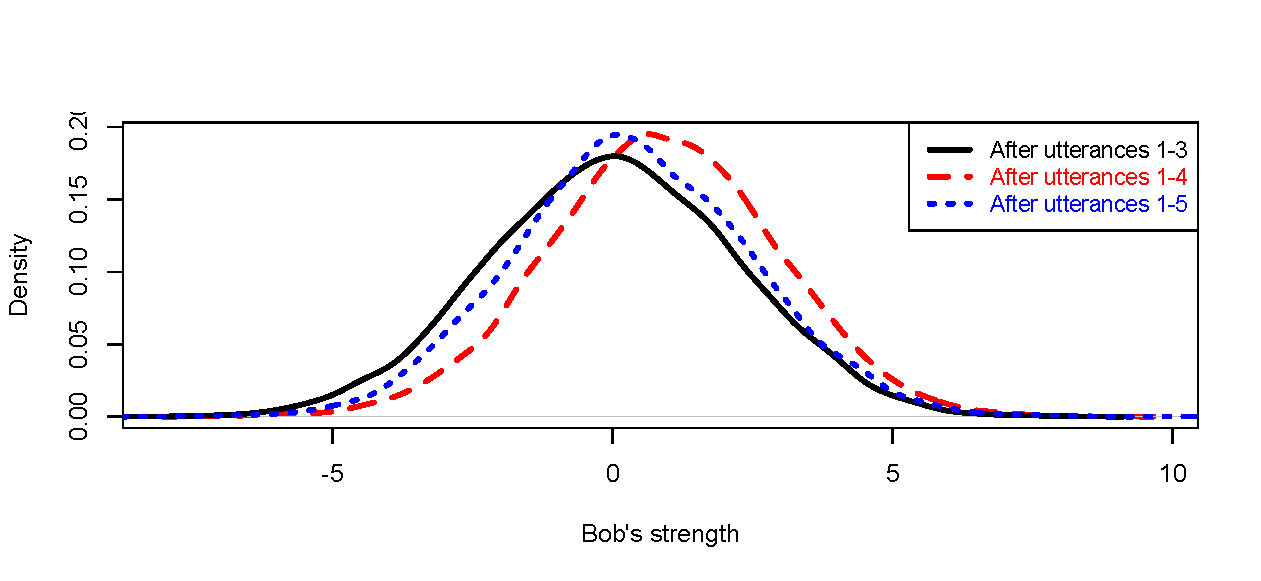
\includegraphics[scale=.65]{explaining-away-ling.pdf}
\end{center}
\caption{A linguistic example of explaining away, demonstrating that the literal listener makes non-monotonic inferences about the answer to the QUD ``How strong is Bob?'' given the utterances described in the main text. 
Lines show the probability density of answers to this QUD after (a) utterances 1-3 (solid); (b) utterances 1-4 (long dash); (c) utterances 1-5 (short dash).}
\end{figure}
Note, however, that this non-monotonic effect comes about not by directly observing a low value for the strength of Bob's opponent Jim as in our earlier example, but by conditioning on the truth of an utterance which does not entail \emph{any} precise value of Jim's strength. 
That is, because there is uncertainty about the strengths of all players, in principle Jim could be the weakest player even he is quite strong, as long as all the other players are strong as well. 
However, the utterance is more likely to be true if Jim's strength falls into the lower tail of the prior distribution. 
Conditioning via \lstinline{query} automatically integrates these two sources of uncertainty, concluding that utterance 5 favors low values of \lstinline{(strength `Jim)} and adjusting the inferred strength of his opponent Bob accordingly. 

\subsection{Ambiguity}
The \lstinline{meaning} function will frequently associate utterances with multiple interpretations. Ambiguities can arise due to any of the following:
\begin{itemize}
\item Syntactic: \lstinline{random-split} will generate possibly different syntactic structures for an utterance on each evaluation. 
If more than one of these structures is interpretable using the composition operators available, the literal listener may entertain interpretations with different syntactic structures.
\item Compositional: Holding the syntactic structure fixed, various choice of composition operators by the \lstinline{random-combinator} function may lead to well-typed outputs. 
Depending on the composition operators available, this may lead to (e.g.) ambiguities of quantifier scope and in whether a pronoun is bound or free.
\item Lexical: the \lstinline{lexicon} function may be stochastic, returning different options for a single item, or words may have intrinsically stochastic meanings (and the former may generally converted to the latter). 
\end{itemize}
One of the crucial advantages of our architecture for language understanding is that these linguistic mechanisms automatically interact with the interpreter's beliefs about the world in an appropriate way. 
When a sentence is ambiguous in any of these ways, the listener will favor plausible interpretations over implausible ones, because the interpreter's model of the world is more likely to generate scenarios which make the sentence true under these interpretations. 
Implausible interpretations, on the other hand, lead to frequent rejection by \lstinline{query} due to their inconsistency with background information.

For example, consider the utterance ``Every player played in some match''. 
Depending on the composition operators used by the \lstinline{meaning} function in a given application, two interpretations are possible:\footnote{As mentioned above, we use the type-shifting mechanisms described in \citet{hendriks93,barker05} to generate this ambiguity from the given utterance.
Note that in the approach described here the composition operations always combine the meanings of two syntactic sisters. 
This means that the set of composition operators must include variants of forward and backward application and composition which apply one or more of Hendriks' unary type-shifting operators to their arguments.
%
% give an example - AR 
%
}
\begin{itemize}
\item ``For every player $x$, there was a match $y$ such that $x$ played in $y$.'' 
\item ``For some match $y$, every player played in $y$.''
\end{itemize}
We can manipulate the plausibility of each of these interpretations by varying the number of players on each team, the number of matches, and the mechanism by which teams are selected to play in matches. 
At one extreme, suppose that the listener has observed that each team has two individuals in it and  (as the theory in Figure \ref{theory} already implies) that only two matches was played:
\begin{lstlisting}
(query
  ...ToW theory...
  (eval QUD)
  (and 
    (= team-size 2)
    (eval (meaning `(every player played in some match)))))
\end{lstlisting}

%
% cont from here
% 

This model predicts that structural ambiguities should behave in a similar way. Suppose we were to enrich the ToW model and lexicon to accommodate utterances such as ``Bill hit the player with the ball''. 
With no background information to constrain interpretation, either interpretation of this utterance might be appropriate, and a true ambiguity is felt. 
However, one of the two possible interpretations is more likely to be true than the other, the literal listener will automatically prefer the parse which generates the more probable interpretation.
In the limit, if one interpretation has zero prior probability, the syntactic ambiguity will not be felt because the interpretation that it generates will always be rejected by the \lstinline{query} function embedded in the definition of the literal listener.
The model predicts that these preferences should display continuous variation between the extremes of assigning equal probability to both and assigning probability 1 to one parse.
Psycholinguistic evidence supports the claim that background information affects the syntactic structures assigned to ambiguous sentences in this way \citep{crainsteedman85,altmannsteedman88,spiveyetal02}.

Lexical uncertainty will not be our focus here, but we should mention two prominent cases: lexical ambiguity and graded meanings. 
Lexical ambiguities of the ``bank''/``bank'' variety could be treated either by having the \lstinline{lexicon} function map ``bank'' to either of two discrete meanings, or by assuming that the latent mechanism which divides utterances into words recognizes two distinct words with this phonological realization.
Intrinsically graded (e.g., prototype) meanings are most naturally thought of as stochastically denoting regions of a non-discrete conceptual space. 
\todo[inline]{Just a quick first pass --- Noah, I suspect you'll want to have a look at this paragraph, and section, and put your own spin on it.}

\subsection{Probabilistic meanings}
 \todo[inline]{This section may be vestigial. it would be nice to somewhere mention that rescaling beliefs is a general mechanism, and that this is equivalent to query. Maybe put this wherever we discuss sequential conditioning as way to update on several sentences...} 
Note that any transition from distribution $P_{\text{before}}$ to distribution $P_{\text{after}}$ such that the support (i.e.\ region of non-zero probability) of $P_{\text{after}}$ is a subset of the support of $P_{\text{after}}$ can be written as multiplying by a real-valued function and then renormalizing. 
That is, any belief update of this type can be written as the result of conditioning on some proposition.


\subsection{Composition}
\todo[inline]{Noah: discuss that compositionality in language and thought are similar but along different `directions'...}
\todo[inline]{Here or maybe in GD: Types useful in SLC but not in LC. (Eg potential locus of asymmetry between kinds and properties?)}

%\item  Sentence meanings: in formal semantics there are two views of meaning. the belief update view (roughly, dynamic semantics) and the intensions---functions from world to truth---view (the Montague, Lewis, etc view). Which is ``correct''? What's the relationship between belief and truth?


%\item Bayesian belief update is via conditioning, conditions are intensions (fns from env/world to truth). So there is a natural probabilistic view that treats meaning as both truth-functional intention and operator of belief update.
%   (Note: any update of a distribution to another that doesn't make certain things uncertain can be represented as conditioning on a stochastic predicate. 
%    Note, environment is natural notion of world... too weird for linguists?
%    Note: introduce SF to LF translation function here.)


%\begin{itemize}  
%\item  Bayesian belief update as the basic operation of literal meaning.
%\subitem     Conservative version uses standard deterministic semantics (world->truth) to update a prior distribution over worlds.
%\subitem     Generative world model has (at least) entities (objects, events, agents, ..) and properties. Recall tug-of-war world.
%\subitem     Consequences:  Graded and non-monotonic effects: 
%"in match1 bob played against jim. bob won match1." ... "jim is the weakest player." : initial graded inference about bob's strength. explaining away. initially think bob strong, then probably not. effect of prior knowledge on these inferences: number of other players and strength variance.
%

%\item  Allow meanings to be non-deterministic themselves (i.e. world->score, or stochastic world->truth).
%\subitem     Consequences: 'Prototype'-like meanings? Soft meaning constraints ("flip him over").
%\subitem     Ambiguity:  homonomy/polysemy, structural ambiguity, scope ambiguity 
%\subitem     Example: manipulate prior for number of players in a match / number of matches on a day... "every player in the league was in a match on tuesday".
%\subitem     Stochastic meaning function or underspecified semantics? equivalent wrt distribution on interpretations.
%\subitem     Mention puns..??
        
%\item  Compositional semantics for stochastic meanings via SLC.
%\subitem     Types useful in SLC but not in LC. (Eg potential locus of asymmetry between kinds and properties?)
%
%\end{itemize}

% \todo{Language and reference variables? Where do we need to introduce reference variables? meaning of "a", "the", "he", etc? only where standard semantics has existentials? any NP (e.g. any specifier)? }


\section{Pragmatic interpretation}

The \lstinline{literal-listener} described above treats utterances as true information about the world, updating her beliefs accordingly. 
In real language understanding, however, utterances are taken as speech acts that inform the listener indirectly by conveying a speaker's intention. In this section we describe a version of the \emph{rational speech acts} model \cite{Goodman2013, Frank2012}, in which a sophisticated listener reasons about the intention of an informative speaker.

First, imagine a speaker who wishes to convey that the question under discussion (\lstinline{QUD}) has a particular answer (or value). This can be viewed as an inference: what utterance is most likely to lead the (literal) listener to the correct interpretation?
\begin{lstlisting}
(define (speaker val QUD)
  (query
    (define utterance (language-prior))
    utterance
    (equal? val (literal-listener utterance QUD))))
\end{lstlisting}
The \lstinline{language-prior} forms the \emph{a priori} (non-contextual and non-semantic) distribution over linguistic forms, which may be modeled with a probabilistic context free grammar or similar model. 
This prior inserts a \emph{cost} for each utterance: using a less likely utterance will be dispreferred \emph{a priori}.
It is clarifying to write the distribution implied by the \lstinline{speaker} function explicitly:
\begin{align}
P(\texttt{ut} | \texttt{val}, \texttt{QUD}) &\propto P(\texttt{ut}) P_{\texttt{listener}}(\texttt{val} | \texttt{ut}, \texttt{QUD}) \\
&\propto e^{\ln(P_{\texttt{listener}}(\texttt{val} | \texttt{ut}, \texttt{QUD})) + \ln{P(\texttt{ut})}}
\end{align}
Thus, the \lstinline{speaker} function describes a speaker who uses a soft-max rule \cite{luce59,suttonbarto98} to choose utterances according to a utility function which is the sum of utterance cost and informativity of the utterance about the \lstinline{QUD} (formalized as negative surprisal of the intended value)\footnote{This formulation is soft-max with parameter $1$, it can be modified to give an arbitrary parameter.}.

A more sophisticated, pragmatic, listener can now be modeled as a Bayesian agent updating her belief about the value of the question under discussion given the observation that the speaker has bothered to make a particular speech act:
\begin{lstlisting}
(define (listener utterance QUD)
  (query
    ...theory...
    (define val (eval QUD))
    val
    (equal? utterance (speaker val QUD))))
\end{lstlisting}
Notice that the prior over \lstinline{val} comes from evaluating the \lstinline{QUD} expression given the \lstinline{theory}, and the posterior comes from updating this prior given that the speaker has chosen \lstinline{utterance} to convey \lstinline{val}.
The force of this model comes from the ability to call the \lstinline{query} function within itself \cite{Stuhlmueller2013}---each query models the inference made by one (imagined) communicator and together they capture sophisticated pragmatic reasoning. 
Several observations are worth making: First, alternative utterances will enter into the computation in sampling (or determining the probability of) the actual utterance from \lstinline{speaker}. Similarly, alternative values are considered in the listener functions.
Second, the notion of informativity captured in the \lstinline{speaker} model is not simply information transmitted by \lstinline{utterance}, but is \emph{new} information conveyed to the listener \emph{about} the \lstinline{QUD}. 
Information which is not new to the listener or which is not relevant to the \lstinline{QUD} will not count in the speaker's utility.

We illustrate by considering quantity implicatures \cite{??}. 
Take as an example the sentence "some of the women are stronger than jane".
\todo[inline]{Dan: Fill in some not all example.... also do "captain" vs "player"? (would need to make names unavailable for this to work...)}

\todo[inline]{reference via joint inference (effect of prior). FG'12 ref exprs. salience. (lewis "the cat"?)

how about a match between '(bob sue) and '(dude alice), where 'dude is male with unknown name, and the utterance is "he's strong!"... "he" should be interpreted as 'dude since otherwise could have used "Bob". this is just like the FG setup.

then do a version where there are two unnamed males, but only one of them was in the match... salience should enter to set "he" to guy just in a match.
}

\subsection{Extensions and related models}

\todo[inline]{Relation to IBR and game-theoretic pragmatics.}
\todo[inline]{extensions: knowledge (GS12), inferring QUD, more general goals, etc.}
% "team A won some of the matches" : implicature that not all of them, unless speaker had not seen all matches.



\section{Semantic indices}

In formal semantics \cite{montague} sentence meanings are often treated as intensions: functions from semantic indices to truth functions. The semantic theory has nothing to say about how to set these indices, only that they matter and (probably) depend on context. Yet we have already seen that a probabilistic theory of pragmatic interpretation can be used to describe the ways that context influences interpretation. Can we similarly use probabilistic tools to describe the ways that semantic indices are set based on context?
We must first decide how semantic indices should enter into the probabilistic framework presented above (where we have so far treated meanings simply as truth functions). The simplest assumption would be that they are random variables that occur (unbound) in the meaning expression and are reasoned about by the literal listener:
\begin{lstlisting}
(define (literal-listener utterance QUD)
  (query
    ...theory...
    (define index (index-prior))
    (define val (eval QUD))
    val
    (eval (meaning utterance))))
\end{lstlisting}
Here we assume that a lexical item may contain an unbound occurrence of \lstinline{index} which is then bound during interpretation by  the \lstinline{(define index ...)} definition.
Because there is now a joint inference over \lstinline{val} and \lstinline{index}, the index will tend to be set such that the utterance is most likely to be true. 
To be concrete, consider the case of gradeable adjectives like \emph{strong}. In section \ref{lexicon} we have defined \sv{strong} = \lstinline[mathescape]{($\lambda$ (x) ($\lambda$ (d) (>= (strength x) d)))}, without specifying how \lstinline{d} is bound in sentences such as ``John is strong.'' 
We could instead define \sv{strong} = \lstinline[mathescape]{($\lambda$ (x) (>= (strength x) d))}, allowing \lstinline{d} to be a free semantic index variable.\footnote{We would then have to make a corresponding change
to the meaning of \emph{-est}: it would first bind the degree locally, then proceeded as above to saturate the threshold.}
 After applying the \lstinline{meaning} function (and simplifying composition) the utterance ``John is strong'' (with \lstinline{QUD} ``how strong is John?'') would be interpreted via:
\begin{lstlisting}
(query
  ...theory...
  (define d (uniform))
  (define val (strength 'John))
  val
  (>= (strength 'John) d))
\end{lstlisting}
To understand this distribution, we can look at the prior (marginal) distributions over \lstinline{d} and John's strength, and the corresponding posteriors.
<<<<<<< HEAD
\todo{Run this simulation. Put in figure. (Note, we want this for SALT paper too!)}
The threshold variable has been influenced by context as expected: it changes from its prior to a posterior that makes the utterance likely to be true. However, this gives us the wrong interpretation of ``John is strong''! What is missing is the pressure to adjust \lstinline{d} so that the sentence is not only true, but also \emph{informative}. 
=======
\todo{Dan: Run this simulation. Put in figure. (Note, we want this for SALT paper too!)}
The threshold variable has been influenced by context as expected: it changes from its prior to a posterior that makes the utterance likely to be true. However, this gives us the wrong interpretation of ``John is strong''! What is missing is the pressure to adjust \lstinline{d} so that the sentence is not only true, but also \emph{informative}. 
>>>>>>> dfa862309b1f1d964af3df7da14821df8b538c1e

Simply including the informative speaker and pragmatic listener models as defined above is not enough: without additional changes the index variables will still be inferred at the level of literal listener with no pragmatic pressures. \todo{Dan: verify that claim. put in simulation result if its interesting..} Instead, we lift the index variables to the pragmatic level. Imagine a pragmatic listener who believes that the index variables have values that she happens not to know, but which are otherwise common knowledge (i.e. known by the speaker, who assumes they are known by the listener):
\begin{lstlisting}
(define (listener utterance QUD)
  (query
    ...theory...
    (define index (index-prior))
    (define val (eval QUD))
    val
    (equal? utterance (speaker val QUD index))))
    
(define (speaker val QUD index)
  (query
    (define utterance (language-prior))
    utterance
    (equal? val (literal-listener utterance QUD index))))

(define (literal-listener utterance QUD index)
  (query
    ...theory...
    (define val (eval QUD))
    val
    (eval (meaning utterance index))))
\end{lstlisting}\footnote{For simplicity we are assuming that it is clear from the argument structure whether the version of each function with or without indices is intended.}
In most ways this is a very small change to the model, but it has important consequences. At a high level, the effect is that index variables will now be set in such a way that they both make the utterance likely to be true \emph{and} likely to be pragmatically useful (informative, relevant, etc); the tradeoff between these two factors results in significant contextual flexibility of the interpreted meaning. In the case of the adjective \emph{strong} we see \todo{put in model figure} that the threshold is now interpreted as roughly one standard deviation from the prior mean strength---hence \emph{strong} means significantly stronger than average, but does not require maximal strength (most informative) or permit any strength (most often true). This model of gradeable adjective interpretation (which was introduced in \cite{Lassiter2013}) has a number of appealing properties: for instance, it explains how background knowledge affects qualitative and quantitative aspects of adjective interpretation (see \cite{Lassiter2013}), and it explains why adjectives result in vaguest interpretation (see below).

We can motivate from this example a general treatment of semantic indices: lift each index into the pragmatic inference, allowing them to bind free variables in the literal meaning, and reasoning over them jointly with world states. 
When we don't know ahead of time which index variables will occur in the literal-listener utterance we need to generalize the above. 
One way is to treat \lstinline{index} as a memoized function mapping variable names to (random) values appropriate for their types.\footnote{The semantics of a memoized function is such that its value on all inputs is formally (if not actually) fixed when the function is created. Thus a memoized \lstinline{index} function would result in index variables that are reasoned about at the pragmatic listener level, although they are made only as needed in the literal listener.} 
Then either the lexical entires should change from free variables to lookups (e.g. \lstinline{d} to \lstinline{(index d)}) or the meaning function is responsible for detecting unbound variables and decorating them with \lstinline[mathescape]{(index ...)}.

Another interpretation of this modeling approach (indeed, the original interpretation, introduced in \cite{Bergen2012}) is as the result of \emph{lexical uncertainty}: each index represents a lingering uncertainty about word meaning (in context) which the listener must incorporate in the interpretation process. This interpretation is appealing in that it connects naturally to language acquisition and change \cite{SmithFrankGoodman}. For instance, upon hearing a new word a learner would initially treat it as underdetermined (essentially an index variables ranging over all expressions of the appropriate type), inferring its meaning on each usage from contextual cues. Over time the prior over this `index' would tighten until only the correct meaning remained, and no contextual flexibility was left. A difficulty with the lexical uncertainty interpretation is explaining why certain aspects of a word's meaning are so much more flexible than others. This is natural from the free-index interpretation since the dimensions of flexibility are explicitly represented as unbound variables in lexical entries. A more structured (e.g. hierarchical) notion of lexical uncertainty may be able to reconcile these interpretations, which are essential equivalent.


\subsection{Other applications of index variables}



\todo[inline]{Discuss Horn implicatures:  Marked meanings and marked utterances: why basic model fails. Then discuss the Bergen results. example in tug-of-war domain?}

% Lifting assignment fn to pragmatic listener. Semantic "existence" or "skolem" operator.  (Why do this and what should lift? Conventional vs coordinated indices? Lexical uncertainty?)

\begin{itemize}
\item horn implicature
\item  "the" vs "a": same basic meaning, but the variable from "the" is lifted to L1, hence is influenced by salience. (competition between "a" and "the"?)
\subitem \sv{the} = \lstinline{($\lambda$ (P) ($\lambda (x) (P x)))}, with the variable $x$ lifted up to the pragmatic listener. 
\item  presupposition accommodation: "the strong player" == the strongest.
\item quantifier scope??
\end{itemize}

\subsection{Vagueness}


\todo[inline]{Dan: Discuss vagueness more generally. Sorites.}







\section{Conclusion}
\begin{itemize}
\item  Kinds of variables: discrete, ordered, and continuous variables.
\item  Roles for uncertainty: world knowledge, SF to LF translation, stochastic meanings, pragmatic coordination.
\item  Pervasive uncertainty and joint inference: understanding is analyzable but not modular.
\end{itemize}






\appendix


\section{Example sentences}
\begin{itemize}
\item "the teams in match1 were bob and jim. bob won match1." ... "jim is the weakest player." : initial graded inference about bob's strength. explaining away. initially think bob strong, then probably not.
\subitem \textsv{the teams in match1 were bob and jim}= \lstinline{(equal? (teams-in-match `match1) `((Bob) (Jim)))}. (Note converting each person into the set which is his team....)
\subitem \textsv{bob won match1}= \lstinline{(equal? (winner `match1) `(Bob))} (Note again converting Bob to his team.)
\subitem \textsv{jim is the weakest player}= \lstinline{(equal? 'Jim (est (< (strength x) t) players))}  (Est has to grab the threshold and set it to highest value s.t. set is non-empty.) 


%\item  "teamA won match 3"
\item : some noun with graded  prototype extent?
\item "every player was in a match yesterday" : scope ambiguity treated either as stochastic meaning fn or underspecified semantics. manipulate priors...
%\item ("the match was aweful/awful for team A" : ambiguous homonym?)
\item "teamA has two players. one is the captain. that player on teamA is strong." : implicates not talking about the captain?  FG'12 style ad-hoc implicature.
%\item "a player on team A is strong" : implicature that not talking about the team captain???
%\item "the player" : salience and definite reference. (something about lewis and cats??)
\item "some of the women are stronger than jane" : implicature that not all of them are.
\item "team A won some of the matches" : implicature that not all of them, unless speaker had not seen all matches.
\item "team A won the match" vs "team A prevailed in the match" : example of horn implicature.. latter implies close match? (need notion of how close the match was?)
     		% closeness = smallness of difference in score
\item "john is strong" : gradable, depends on prior over strengths.
\item "the strong player" : interpreted as strongest by joint inference of threshold and reference.
\item "john is strong, jim is a little less strong. is jim strong?" : sorites.
\end{itemize}



\section{Modeling sketch}

\begin{table}[htdp]
\caption{default}
\begin{center}
\begin{tabular}{llc}
\sv{`players}&= & $`(Bob\ Jim ...)$ \\
\sv{`Bob}&= & $`Bob$ or $`(Bob)$ \\
\sv{player}&= & $\lambda.x (x\in players) $ \\
 
\end{tabular}
\end{center}
\label{default}
\end{table}%



\noindent Basic ontology: 
\begin{itemize}
\item players: some humans
\item strength and other properties of people.
\item the set of teams: a partition of the set of players, each associated with a unique name (a capital letter) and a distinguished player (the captain)
\item matches: a set of data structures consisting of an integer (the match number), 2 teams, and a winner
\item $D_e: \{x|\mathit{player}(x)\} \cup \{x|\mathit{match}(x)\} \cup \{x|\mathit{team}(x)\}$
\item $D_t = \{0,1\}$
\item $D_d = (0,1)$
\end{itemize}

\noindent Vocabulary:
\begin{itemize}
\item some names of individual players which we set out stipulatively, and the set of players (or people).
\item player: function from individuals (names) to $\{0,1\}$
\item men, women: function from individuals (names) to $\{0,1\}$, constrained so that $\mathit{player}(x) \rightarrow \mathit{man}(x) \vee \mathit{woman}(x)$
\item captain: function from teams t to functions from individuals x to 1 if x is t's captain, else 0
\item match: a function $D_e \rightarrow \{0,1\}$, true of matches only, with an optional integer argument (since we want both \emph{a match} and \emph{in match n}) 
\item play: a function from an integer n and two teams x,y to $\{0,1\}$: x played y in match n
\item win: $\mathit{win}(y)(x)$ is true iff y is a match and x is the winner in y
\item team: a set of players
\item strength: function from players to $(0,1)$, Gaussian prior (separate priors for men and woman would be useful but perhaps unnecessarily controversial)
\item $\theta_A$: free variables with $\mathcal{U}(0,1)$ prior, one for each adjective $A$
\item a, some of: $\lambda P \lambda Q . \exists x P(x) \wedge Q(x)$
\item every/all of: $\lambda P \lambda Q . \forall x P(x) \rightarrow Q(x)$
\item quantifier scope ambiguities: I think we should just give the truth-conditions of the two interpretations, mention various options for computing them but not commit to one. [The key is just that both options are possible interpretations and the pragmatic listener optimizes the probability of the disambiguated utterance given the speaker model; the mechanism for generating the LFs probably isn't important.]
\item strong: $\lambda x . \mathit{strength}(x) > \theta_{\mathit{strong}}$
\item score1, score2: auxiliary functions with apply to a match and return the score of the team listed first/second 
\item close: $\lambda x . \mathit{match}(x): \mathit{score1}(x) - \mathit{score2}(x)| < \theta_{\mathit{close}}$ [presupposes argument is a match, asserts it was theta-close]
\item the: a choice function, i.e., a function from a property to some individual who satisfies the property; the prior distribution is uniform over all individuals who have the property. (The graded salience effects should kick in at L1, in reasoning about who its more likely that the speaker would be talking about.)
\item less: a function from an adjective (\emph{close, strong}) and a degree $d$ to properties of individuals $x$, returning true iff the adjective holds of $x$ to a degree less than $d - \epsilon$. By default, $r = 0$. 
\item A little: a modifier of \emph{less} s.t.\ , where epsilon is a free parameter which we can vary to make the point about how the sorites works.
\item -est: function from domains and adjectives to adjectives, where the latter is true only of individuals with argmax degree of the property in the domain
\item a little: make this a vocabulary item  
\end{itemize} 



%
%
%\section{Old stuff we may want to draw on...}
%
%%%"The major portion of the proposal should consist of a clear description of the technical approach being proposed. This discussion should provide the technical foundation/justification for pursuing this particular approach/direction and why one could expect it to enable the objectives of the proposal to be met."
%
%Words are potentially one of the clearest windows on human knowledge and conceptual structure. If we understood the connection between words and mental representation, we could gain critical insights into almost every aspect of psychology, construct vastly more useful thinking machines, and interface the two. But what do words mean? In this project we aim to {\bf construct and explore a formal model of lexical semantics grounded, via pragmatic inference, in core conceptual structures}. We will do so using a set of modeling tools---chiefly the probabilistic programming language Church \cite{goodman2008}---that we have previously developed and used to explain  aspects of high-level human cognition.
%
%Flexible human cognition is derived in large part from our ability to imagine (or sample, or simulate) possible worlds. A rich set of concepts, intuitive theories, and other mental representations support imagining and reasoning about possible worlds---together we call these {\bf core cognition}\footnote{This phrase is chosen to connote the \emph{conceptual core} of human thinking, in contrast to the distal processes of low-level perception, attention, etc. There is no particular connection intended to the developmental claims of \emph{core knowledge}, except for a concern with concepts and high-level cognition.}. We can formalize key pieces of core cognition (such as intuitive physics and theory of mind) using probabilistic programming tools, developed in previous ONR-funded research  (``A framework for core cognition'', ONR N00014-09-1-0124), by viewing commonsense knowledge as a set of interrelated definitions (or concepts) in a probabilistic programming language. Probabilistic programs specify sampling procedures over possible program executions, each execution fixes (some of) the variables in that describe the world, hence each collection of concepts describes how to sample from a rich space of possible worlds. The inference (or conditioning, or query) operator describes how to use these distributions on worlds for reasoning.
%We have been able to explain many inferences that humans draw from sparse evidence using these tools. Here we posit that this collection of concepts also forms the set of primitive elements available for {\bf lexical semantics}: word meanings can be built from the pieces of core cognition.
%
%However, the connection between core concepts and lexical semantics is not direct: 
%first, 
%because language must flexibly adapt to the context of communication, the connection between lexical representation and interpreted meaning is mediated by pragmatic inference;
%second, 
%sentence meanings act as constraints on possible worlds, via their truth-value, whereas core concepts describe generation of possible worlds.
%%
%% [DL] I think the previous clause may be somewhat difficult to understand for people who don't know about our angle yet...
%%
%We propose to explore a model of language that formalizes and explains these differences, again using tools of probabilistic programming. 
%
%In recent work we have made preliminary progress at combining underspecified semantic representations with a general purpose pragmatic inference mechanism.
%This potentially allows us to account for subtle aspects of language use with relatively simple semantic denotations.
%%: aspects of conveyed meaning emerge from an interaction of semantic denotation with context and core conceptual structures.
%In particular, we view semantic representation as indivisible from core cognition, and the effective meaning of words as emerging from a pragmatic inference process. A synergistic ONR project (``Grounded language understanding as social cognition'', PI Chris Potts) proposes to study the details of the pragmatic mechanism. In particular, this related project will perform detailed experimental studies of coordination games, which model pragmatics with minimal need for semantics---thus verifying the pragmatic framework used here to support our investigations of lexical semantics.
%
%Our approach is similar in spirit to cognitive semantics, in that we attempt to ground semantics in mental representation, but we draw on the highly successful tools of Bayesian cognitive science to formalize these ideas. 
%Similarly, our approach draws heavily on the progress made in formal model-theoretic semantics \cite{montague1973,heimkratzer1998}, borrowing insights about how syntax drives semantic composition, but we compose elements of stochastic logics rather than deterministic ones.
%Finally, our approach is related to recent progress in robotics (and indeed our project will benefit from ongoing collaboration with roboticist Stefanie Tellex of Brown University), but is more systematic and systematically connected to cognitive and linguistic theory. 
%
%We propose to study lexical semantics in the setting of an architecture for language understanding that is described in section \ref{langaugemodels}. We first provide, in section \ref{background}, background on the probabilistic programming language Church and on using Church to describe core cognition. In section \ref{lex} we describe the case studies of lexical semantics that we propose to explore in this project. We will rely heavily on computational infrastructure for inference in the Church language; the models we propose push the envelope of what is currently possible and will require new inference techniques. In section \ref{infrastr} we describe proposed work on Church inference algorithms and implementations.
%
%
%\section{Commonsense reasoning}
%\label{background}
%
%Probabilities describe degrees of belief, and probabilistic inference describes rational reasoning under uncertainty. It is no wonder, then, that probabilistic models have exploded onto the scene of modern artificial intelligence, cognitive science, and applied statistics: these are all sciences of inference under uncertainty. But as probabilistic models have become more sophisticated, the tools to formally describe them and to perform probabilistic inference have wrestled with new complexity. Just as programming more than the simplest algorithms requires tools for abstraction and composition, complex probabilistic modeling requires new progress in model representation---\emph{probabilistic} programming languages. These languages provide compositional means for describing complex probability distributions; implementations of these languages provide \emph{generic} inference engines: tools for performing efficient probabilistic inference over an arbitrary program. 
%
%By providing a uniform and universal representation for probabilistic models, probabilistic programming provides a framework for unifying disparate Bayesian models of human cognition. Indeed, while Bayesian models have been extremely influential in cognitive science \cite[e.g.][]{tenenbaum2011}, 
%%
%% do you want ``How to grow a mind''? It's in the bib now as tenenbaum2011.
%%
%it is only recently that we have the tools to view the Bayesian approach as a general framework for mental representation.
%We next give a brief introduction to probabilistic programming, then an indication of how these tools can be used for modeling human cognition.
%
%\subsection{Probabilistic Programming Languages and Church}
%
%In their simplest form, probabilistic programming languages extend a well-specified deterministic programming language with primitive constructs for random choice. 
%This is a relatively old idea, with foundational work by Giry, Kozen, Jones, Moggi, Saheb-Djahromi, Plotkin, and others \cite[see e.g.][]{JP89}. Yet it has seen a resurgence thanks to new tools for probabilistic inference and new complexity of probabilistic modeling applications. There are a number of recent probabilistic programming languages \cite[e.g.][]{sato97,Pfeffer01,milch05,richardson06,Poole:2008wk,kiselyovS09,Pfeffer:2009wo,mccallum2009factorie,Kimmig:2011tn}
%embodying different tradeoffs in expressivity, efficiency, and perspicuity. 
%We will focus on the probabilistic programming language Church  \cite{goodman2008}, which has the benefits of being close to the core mathematical foundation (stochastic lambda calculus) yet having sufficient expressivity to easily represent abstract structures needed in cognitive modeling.
%
%Church extends (the purely functional subset of) Scheme \cite{Abelson1996} with elementary random primitives, such as \lstinline{flip} (a bernoulli), \lstinline{multinomial}, and \lstinline{gaussian}. In addition, Church includes language constructs that simplify modeling. For instance, \lstinline{mem}, a higher-order procedure that memoizes its input function, is useful for describing persistent random properties and lazy model construction. %(Interestingly, memoization has a semantic effect in probabilistic languages.)
%If we view the semantics of the underlying deterministic language as a map from programs to executions of the program, the semantics of the probabilistic language is a map from programs to distributions over executions. When the program halts with probability one, this induces a proper distribution over return values. Indeed, \emph{any} computable distribution can be represented as the distribution induced by a Church program in this way (see \cite[\S6]{Freer2012}, \cite[\S11]{ackerman2011}, and citations therein).
%
%%Probabilistic graphical models  \cite{koller2009}, aka Bayes nets, are one of the most important ideas of modern AI.
%Probabilistic programs extend probabilistic graphical models \cite{koller2009}, aka Bayes nets, one of the most important ideas of modern AI. Indeed, graphical models can be seen as flow diagrams for probabilistic programs---and just as flow diagrams for deterministic programs are useful but not powerful enough to represent general computation, graphical models are a useful but incomplete approach to probabilistic modeling. For an example of this, we need look no further than the fundamental operation for inference, probabilistic conditioning, which forms a posterior distribution from the prior distribution. Conditioning is typically viewed as a special operation that happens \emph{to} a probabilistic model (capturing observations or assumptions), not one that can be expressed \emph{as} a model. However, because probabilistic programs allow \emph{stochastic recursion}, conditioning can be defined as an ordinary probabilistic function (Fig.~\ref{query}, Top). 
%%(However see \cite{ackerman2011} for complications in the case of continuous values.) 
%Notice that, since conditioning is an ordinary function, conditioning can be nested inside other calls to the conditioning operator. This is a pattern that we will use in defining our language models in section \ref{langaugemodels}.
%
%In Church, conditioning is specified by the more convenient \lstinline{query} syntax (Fig.~\ref{query}, Bottom). A Church query first gives a set of stochastic function definitions, which set up the ``language'' of the query, then gives the query expression (whose value we will return) and finally the condition expression, which must return true. We also allow \lstinline{factor} statements which provide another way of constraining a query: the statement\\ \lstinline{(factor expr)} multiplies the value of \lstinline{expr} (assumed to be a real number) into the probability of the current execution. This provides a convenient way to add a soft constraint on the distribution of executions (via a side-effecting operation).
%
%\begin{figure}[tbp]
%\begin{center}
%
%\begin{minipage}[b]{0.7\linewidth}
%
%\begin{lstlisting}
%(define (rejection-query thunk condition)
%  (let ((val (thunk)))
%    (if (condition val)
%        val
%        (rejection-query thunk condition))))
%\end{lstlisting}
%\end{minipage}
%
%
%\begin{minipage}[b]{0.3\linewidth}
%\begin{lstlisting}
%(query
%  ...defines...
%  query-expression
%  condition-expression)
%\end{lstlisting}
%\end{minipage}
%\hspace{2em}
%%$\rightarrow$
%\begin{minipage}[b]{0.3\linewidth}
%\begin{lstlisting}
%(define (thunk)
%  ...defines...
%  (pair query-expression
%     condition-expression))
%(define condition rest)
%\end{lstlisting}
%\end{minipage}
%
%\caption{(Top) Defining conditional inference in Church as a stochastic recursion: rejection sampling represents the conditional probability of the thunk conditioned on the condition predicate being true. We typically use special query syntax (Bottom, left), which can be desugared into a query thunk (Bottom, right).}
%\label{query}
%\end{center}
%\end{figure}
%
%
%
%\begin{figure}[htbp]
%\begin{center}
%
%(a)\\
%\begin{minipage}[b]{0.7\linewidth}
%\begin{lstlisting}[mathescape]
%;;Strength is a persistent (memoized) property of each person:
%(define strength (mem (lambda (person) (gaussian 1.0 1.0))))
%
%;;Laziness varies from match to match:
%(define (lazy person) (flip 0.3))
%
%;;When a person is lazy they pull less:
%(define (pulling person) (if (lazy person) 
%                             (/ (strength person) 2) 
%                             (strength person)))
%
%;;Total pulling of the team is the sum:
%(define (total-pulling team) (sum (map pulling team)))
%          
%;;The winning team pulls hardest:    
%(define (winner team1 team2) 
%  (if ($<$ (total-pulling team1) (total-pulling team2)) 
%      team2 
%      team1))
%\end{lstlisting}
%\end{minipage}\\
%(b)\\
%\includegraphics*[scale=0.5]{BPPexpt1}
%
%\caption{Modeling intuitive concepts in the tug-of-war domain. (a) A Church model to capture core concepts.  While this model is simple, probabilistic queries can explain human reasoning from diverse evidence with high quantitative accuracy. (b) Comparison of the model to human judgements in Experiment 1 of \cite{gerstenberg2012}.}
%\label{tug}
%\end{center}
%\end{figure}
%
%
%
%\subsection{Core Cognition: Intuitive Theories and Conceptual Structure}
%
%Church programs can be used to express a wide variety of cognitive models, capturing concepts from core cognitive domains and core concepts from many specific areas of knowledge. For a complete tutorial on using Church to model human cognition, including many  examples, see \url{http://www.stanford.edu/~ngoodman/ProbMods.html}.
%
%To illustrate, we consider the problem of capturing commonsense knowledge about the game tug-of-war. Figure \ref{tug}a, gives Church functions specifying key concepts for this domain (though certainly not exhausting possible knowledge about the game). This ``conceptual library'' of probabilistic functions can be used to reason about many patterns of evidence, via different queries, without needing to specify ahead of time the set of people, the teams, or the matches. 
%A Church program provides a description of how to go about simulating a possible world in the domain (here, randomly choosing strengths, laziness, etc., and computing the winner of each match). To reason from evidence or hypotheses, this simulation process is directed: a query describes what assumptions to fix and what to simulate (for instance, fixing match outcomes and simulating strengths). 
%%The program thus enables a very large numbers of different inferences to be modeled. 
%%The ability to model many inferences is inherited from the productivity of the underlying programming language, while the ability to capture complex, graded commonsense reasoning is inherited from probabilistic inference by simulation.
%
%The predictions of this simple model match human intuitions quite well, Figure \ref{tug}b. In \cite{gerstenberg2012} we presented people with the results of a set of matches in a ``ping-pong tournament'', and asked for judgements about the strength of one of the players.
%We found a correlation of 0.98 between model and human judgements. This compelling fit suggests that the definitions in Figure \ref{tug}a capture important aspects of the concepts people have for reasoning about team games. However, connecting these concepts to natural language would provide a much more natural probe of people's intuitions. For instance, we would like to ask \emph{Is Bob strong?}~rather than asking for an arbitrary rating of Bob's strength; but how does the adjective \emph{strong} in this positive form relate to the conceptual degree of \lstinline{strength}? The connection must be indirect since, as discussed in section \ref{sec:GA}, a statement like \emph{Bob is strong} can be interpreted very differently in different contexts.
%More generally, how may we use concepts defined in a Church model for a given domain to build the semantics of natural language for this domain?
% 
%
%%\todo{intuitive physics and ToM.}
%
%
%%%%%%%%%%%%%
%
%\section{Literal meaning as conditioning}
%\label{L0}
%
%The basic assumption of our probabilistic model of language interpretation is that sentences can be used to update the listener's belief distribution. Because probabilistic belief update is performed by \emph{conditioning} a prior distribution to get a posterior distribution, the meaning of a sentence should be a conditioning expression---an expression that evaluates to true or false.
%If we assume further that a listener's prior knowledge about the world is given by her concept definitions, then the literal interpretation of language can be given by the Church function: 
%\pagebreak
%\begin{lstlisting}
%;;The basic listener: how is the world, given that the utterance is true?
%(define (L0 utterance QUD)
%  (query
%    ...core concept definitions...
%    (eval QUD)
%    (eval (meaning utterance))))
%\end{lstlisting}
%This describes a listener \lstinline{L0} who hears \lstinline{utterance}, and is interested in the import for a given question-under-discussion\footnote{Conceptually, we think of the listener as forming a distribution over possible worlds. However worlds are unwieldy to represent (being infinitely large), so we represent this distribution instead by a function that can give the distribution over answers to every question that can be asked in a world. This QUD is a notion used widely in formal models of discourse \cite{kuppevelt95,ginzburg95a,ginzburg95b,roberts96,roberts04,beaverclark08}.} 
%(\lstinline{QUD}).
%The (meta-)operator \lstinline{eval} evaluates a given expression in the current environment. Here this means evaluating both the \lstinline{QUD} expression and the meaning of the utterance in an environment in which the core concept definitions are visible.
%The result is a posterior distribution for each possible \lstinline{QUD}---hence a posterior distribution over possible worlds.
% 
%\paragraph{Meaning Composition}
%We assume that the utterance has already been parsed into a syntactic tree. We don't address this syntactic parsing problem in this project, but instead assume it can be effectively handled by existing tools. 
%Following standard practice of formal semantics \cite{heimkratzer1998} we construct the meaning of the sentence recursively along the syntactic tree:
%%
%% DL question: I haven't used SP, but doesn't the fact that it's a dependency parser make it a somewhat poor choice here? There are some option in the linguistics literature (e.g. http://pagesperso.lina.univ-nantes.fr/info/perso/permanents/dikovsky/publies/dgsemantics.pdf), but I think it's considered to be a non-trivial problem. Of course you can throw some fancy machine learning at the problem, e.g. in Percy Liang's stuff, but I don't think the syntax-driven Heim & Kratzer-style approach will work.
%%
%\begin{lstlisting}
%;;Meanings are constructed by recursive composition along the (syntactic) tree:
%(define (meaning utterance)
%  (if (lexical-item? utterance)
%      (lexicon utterance)
%      (pair (meaning (left utterance)) (meaning (right utterance)))))
%\end{lstlisting}  
%Here the predicate \lstinline{lexical-item?} determines if the remaining utterance is a single lexical item (entry in the lexicon), the function \lstinline{left} returns the left subtree of the utterance (which we assume is the operator---possibly through a syntactic transformation), and \lstinline{right} returns the right subtree. By combining meanings with the \lstinline{pair} operator, we are implying that composition happens by function application: when the meaning is evaluated (in \lstinline{L0}) the left subtree meaning will be applied to the right subtree meaning.
%
%
%\paragraph{Lexical Meanings}
%The function \lstinline{lexicon} looks up the meaning of a word, returning an expression that can be evaluated in the current environment. Because this environment contains core concept definitions, the meanings of words can (and will) refer to non-linguistic mental representations: meanings of words are about the possible worlds that a listener considers. The lexicon is described in detail in section \ref{lex}. 
%(In later sections use the standard notation \sv{\mathit{word}} for \lstinline{(lexicon} {\it word}\lstinline{)}.)
%
%
%\subsection{Ambiguity}
%
%  
%\section{L1 Model: Pragmatic enrichment}
%The literal meaning, as encoded by \lstinline{lexicon} and interpreted by \lstinline{L0}, forms the stable contribution of words to meaning across contexts; however meaning can often be strengthened or changed in particular communicative contexts by pragmatic inference.
%Here we model pragmatic enrichment of the literal meaning following \cite{Frank2012,Goodman2013,stuhlmuller2012dynamic}. 
%Critically, because \lstinline{query} is an ordinary function that may be nested in itself, we are able to model a listener reasoning about a speaker, who reasons about a literal listener. This model formalizes the idea that a listener is trying to infer what the speaker intended, while a speaker is trying to make the listener form a particular belief. 
%
%The reflective speaker makes a speech act in order to lead the listener to infer a particular value of the question under discussion:
%\begin{lstlisting}
%;;The speaker: what should I say, so that the listener forms the right interpretation?
%(define (S1 val QUD)
%  (query
%    (define utterance (language-prior))
%    utterance
%    (equal? val (L0 utterance QUD))))
%\end{lstlisting}
%This function describes a soft-max optimal speaker 
%%
%% \cite{luce59,suttonbarto98} ? Might be worth saying in a few words what this means, e.g. ``describes a speaker who uses a soft-max rule \cite{luce59,suttonbarto98} to choose utterances $u$ according to the probability that $u$ will lead the literal listener to the right answer to QUD'' ?
%%
%whose goal is for the literal listener to arrive at a given interpretation. 
%The \lstinline{language-prior} forms the \emph{a priori} (non-contextual and non-semantic) distribution over linguistic forms, which may be modeled with a probabilistic context free grammar or similar model. 
%This prior inserts a \emph{cost} for each utterance: using a less likely utterance will be dispreferred \emph{a priori}.
%%---that is a speaker incurs a cost for using a more complex utterance.
%
%The pragmatic listener can now be modeled as a Bayesian agent inferring the value of the question under discussion, given that the reflective speaker has bothered to make a particular speech act:
%\begin{lstlisting}
%;;The pragmatic listener: what value does the QUD have, given that a speaker chose this utterance to express it?    
%(define (L1 utterance QUD)
%  (query
%    ...core concept definitions...
%    (define val (eval QUD))
%    val
%    (equal? utterance (S1 val QUD))))
%\end{lstlisting}
%This model gives rise to standard scalar implicatures (e.g.~\emph{some} implies \emph{not all}) and has been shown to predict human judgements with high quantitative accuracy in several language understanding tasks \cite{Frank2012,Goodman2013}. Ongoing research aims to further explore the ability of this model to predict human behavior in reference games and simple language understanding tasks.
%
%\subsection{Scalar implicature}
%
%
%
% 
%\section{L1-sv Model: Free semantic variables}
%
%
%\begin{figure}[tbhp]
%\begin{center}
%\begin{minipage}{0.7\linewidth}
%\begin{lstlisting}
%(define (L0 utterance QUD sv)
%  (query
%    ...core concept definitions...
%    (eval QUD)
%    (eval (meaning utterance))))
%
%(define (S1 val QUD sv)
%  (query
%    (define utterance (language-prior))
%    utterance
%    (equal? val (L0 utterance QUD sv))))
%
%(define (L1-sv utterance QUD)
%  (query
%    ...core concept definitions...
%    (define sv (semvar-prior))
%    (define val (eval QUD))
%    val
%    (equal? utterance (S1 val QUD sv))))
%\end{lstlisting}
%\end{minipage}
%\caption{A probabilistic model of natural language understanding incorporating a literal listener \lstinline{L0}, a reflective speaker \lstinline{S1}, and a pragmatic listener \lstinline{L1-sv} who reasons about the question under discussion and the value of free semantic variables.}
%\label{L1-sv}
%\end{center}
%\end{figure}
%
%Under standard linguistic analysis, the literal meaning of a sentence frequently leaves some aspects underspecified; to assign a complete meaning to the sentence, pragmatic inference is required to fill in the value of these \emph{free variables}. This occurs, for example, in sentences such as \emph{He is drinking a martini}, which cannot receive a determinate meaning until the intended referent of \emph{He} is identified (see section \ref{indexicals}). It is believed that the same holds for \emph{Sam is tall}, since literal meaning underdetermines the height required to count as \emph{tall} (see section \ref{sec:GA}); or again for \emph{Moose have horns}, where the semantics does not determine what proportion of moose must have horns in order for this sentence to be true (see section \ref{sec:generics}). This type of context-dependence is widespread in language, but a general and precise framework for understanding how speakers and listeners make use of and resolve underspecified meanings has not previously been proposed.
%
%In our approach, semantic context-dependence is connected with pragmatic inference by instantiating semantic variables at the \lstinline{L1} level and passing them down to lower levels. The complete model is shown in Figure \ref{L1-sv}.
%In this model, a reflective listener \lstinline{L1-sv} evaluates candidate resolutions of the free semantic variables \lstinline{sv} jointly with possible values for the \lstinline{QUD}.
%As we describe in section \ref{lex}, this results in an interaction that produces powerful context-sensitive usage of words despite relatively impoverished semantic representations.
%
%For a fully compositional theory of natural language semantics, a mechanism is needed to account for the fact that expressions with free semantic variables (such as the pronoun \emph{he}) can occur in arbitrarily embedded positions in a sentence.
%Notice that when the \lstinline{QUD} and the meaning of the utterance are evaluated in \lstinline{L0} of this model, they are evaluated in an environment in which the semantic variables (\lstinline{sv}) are bound variables (because these are arguments to the \lstinline{L0} function). These variables are thus free with respect to the lexical entries, but not with respect to the full language model---they have been filled in by the pragmatic listener model. Using an environment to bind the free variables in this way is similar to the approach of relativizing the meaning function to a fixed set of parameters \cite{lewis79,lewis97,barker02}.
%An alternative approach would be to adopt the assumptions about compositionality associated with \emph{variable-free semantics} \citep{szabolcsi87,steedman01,jacobson99,barker07}. In this approach, the standard mechanism of function application is augmented, making it possible to lift a free variable out of deeply embedded syntactic positions, to the top level of literal meaning.
%
%
%%For instance, example \ref{e.1a} is assigned the semantic representation in example \ref{e.1b}, with the variable $x$ representing the pronoun lifted up to the top level despite being buried deeply in the embedded clause.
%%\begin{exe}
%%\ex{\label{e.1} 	 	}
%%\begin{xlist}
%%\ex{\label{e.1a} 	Sam thinks that Bill knows that she is drinking a martini.	}
%%\ex{\label{e.1b} 	$\lambda x : \textbf{female}(x) [\textbf{think}(\textbf{Sam})(\textbf{know}(\textbf{Bill})(\textbf{drinking-a-martini}(x)))]$	}
%%\end{xlist}
%%\end{exe}
%%Similarly, in examples involving gradable adjectives surveyed below the threshold variable $\theta$ is lifted to the top level from arbitrarily embedded positions, as in example \ref{e.2}. 
%%\begin{exe}
%%\ex{\label{e.2} 	 	}
%%\begin{xlist}
%%\ex{\label{e.2a} 	Sam thinks that Bill knows that Mary is tall.	}
%%\ex{\label{e.2b} 	$\lambda \theta [\textbf{think}(\textbf{Sam})(\textbf{know}(\textbf{Bill})(\mathit{height}(\textbf{Mary}) > \theta))]$	}
%%\end{xlist}
%%\end{exe}
%
%
%
%

%%%%%%%%%%%%%
%
%The language architecture described above predicts the interpretation of an utterance given its semantic content and context; fixing the semantic content of particular (classes of) words makes this abstract architecture concrete by grounding language use into the concepts of core cognition. In this section we describe our proposal to study several classes of words as representative case studies in which concepts, uncertainty, and inference interact in important ways. We place particular emphasis on the cases in which free semantic variables are needed to allow contextual flexibility in semantic interpretation.
%
%\subsection{Indexicals and referring expressions}
%\label{indexicals}
%
%Perhaps the simplest case where semantic free variables are needed is in the meanings of referring expressions. 
%For instance, the meaning of \emph{He is drinking a martini} can be taken to be (approximately): $\text{male}(x)\wedge \text{drinking}(x,y) \wedge \text{martini}(y)$, where $x$ and $y$ are free semantic variables that range over individual entities. The semantic contribution of \emph{he} to this meaning is two-fold: it introduces a free variable, and it constrains that free variable to be a male. However, in order to compose properly with the surrounding sentence, the return value of \emph{he} must be only the variable $x$. We can add the constraint, without affecting the return value, by using a Church factor statement: \\
%\indent \sv{\mathit{he}}$=$\lstinline[keepspaces]{(begin (factor (if (male x) 1.0 0.1)) x)}. \\
%This definition adds the constraint as a side-effect, then goes on to return the value of the free variable \lstinline{x}.
%Notice that the constraint that \emph{he} be male is a soft constraint: in a situation where no male referent for $x$ is plausible, it can be interpreted as a non-male. (For instance, in a situation in which we are discussing the best way to cook a burger the sentence \emph{Wait until he's just brown, then flip him} can be interpreted as referring to the burger.) Interpretation of the pronoun is guided by the semantics, but driven by probabilistic inference of the sentence meaning (similar to the conclusion of \citet{kehler08}).
%
%The constraints in this approach are determined by the conceptual content, but so are the potential referents: the possible values of $x$ are not entities in the world, but entities in the possible world represented by the listener \lstinline{L1-sv}. This is particularly striking in the case of
%indexicals such as \emph{I/here/now/that}. The free variable for \emph{now} ranges over times, that for \emph{I} over people, and each must have meta-access to the speech act itself. For instance, \\
%\indent \sv{I}$=$\lstinline[keepspaces]{(begin (factor (if (eq? x (speaker-of utterance)) 1.0 0.1)) x)}; \\
%where we have made use of the fact that the utterance is bound in the environment in which \sv{I} is evaluated (being an argument to \lstinline{L0}), and assumed that the \lstinline{speaker-of} function returns the individual who performed a speech act.
%
%
%Horn's \emph{division of pragmatic labor} \cite{Horn1984} presents a more subtle case for the pragmatic fixing of reference. This principle dictates that, in the absence of distinguishing semantic content, simple utterances should be interpreted as un-marked (i.e.~simple/probable/good) meanings and complex utterances as marked (i.e.~deviant/unlikely/bad) meanings. For instance \emph{I got the car started} is interpreted as doing something unusual to start the car, since the simpler phrase \emph{I started the car} is available to be interpreted as simply turning the ignition.
%To formalize this, imagine cheap/costly utterances \emph{u1}/\emph{u2} and \emph{a priori} likely/unlikely interpretations of the QUD \lstinline{val1}/\lstinline[mathescape]{val2}.
%We would like the less costly expression to be interpreted as the more likely interpretation: 
%\sv{u1}${=}$\lstinline{val1}, \sv{u2}${=}$\lstinline{val2}. 
%This is a simple signaling game \cite{Franke2009}, and this solution is a Nash equilibrium; however, there are many equally good Nash equilibria for this game. A number of attempts have been made to explain why this particular equilibrium should be chosen, but all require ad-hoc stipulations on the equilibrium concept.
%Indeed, the simple model \lstinline{L1}, with no semantic free variables, is unable to arrive at the correct interpretations.
%We have shown in \cite{bergen12} that the \lstinline{L1-sv} model does arrive at the correct interpretations in this case.
%Many questions and difficulties remain to integrate this result with lexical semantics more generally. In particular, how does the division of labor play out in situations with similar but not equivalent semantic meaning, and what semantic work can we rely on this  effect to do?
%
%We propose to use the \lstinline{L1-sv} framework with constrained entity variables to study the details of how referring expressions can be flexibly interpreted. 
%As illustrated above, complex interpretation patterns can be expected as context, concepts, and inference interact.
%We will explore the ways that context allows semantic constraints to be violated, the conceptual grounding of indexicals, the effect of alternative referring expressions, and the use of division of pragmatic labor in simplifying semantic denotations.
%
%
%\subsection{Scalar Adjectives}
%  \label{sec:GA}
%  
%Many words resist simple truth-functions that could be used to tell with certainty when they hold. For instance, exactly how tall must a person be to be a \emph{tall person}?
%Vagueness of meanings has been the subject of much discussion in philosophy and linguistics, and is of critical importance in the psychological literature on graded concepts \cite{rosch78,oshersonsmith81,armstrong83,kamppartee95,fodorlepore96,hampton07}. 
%Vagueness is particularly clear in the meanings of gradable adjectives, such as \emph{tall/short}, \emph{wide/narrow}, \emph{happy/sad}, \emph{wet/dry}, and \emph{full/empty}. 
%These adjectives serve to express measurement along a scale (\emph{Sam is six feet tall}); they are grammatically gradable (\emph{Sam is very tall}), are typically vague, and are highly context-sensitive \cite[e.g.~][]{kamp75,fine75,cresswell76,vonstechow84,williamson94,kennedymcnally05,kennedy07}. 
%%For example:
%%\begin{exe}
%%\ex{\label{e1} 	 Measurement and gradation:		}
%%\begin{xlist}
%%\ex{\label{e1a} 	.	}
%%\ex{\label{e1b} 	This glass is 50\%/completely full.	}
%%\end{xlist}
%%\end{exe}
%
%Vagueness can be seen from the existence of \emph{borderline cases}: individuals for whom it is unclear whether an adjective applies. A seven-foot-tall man is obviously tall, and a five-foot-tall man is obviously not; but does a man who is $6'2''$ count as ``tall''? When asked a question of this type, speakers typically express uncertainty, and show disagreement in responses to a forced-choice \citep{bonini99,schmidtetal09,verheyen10,alxatib11}. 
%The vagueness of adjectives appears to be related to statistical properties of a \emph{comparison class} \citep{bierwisch89,schmidtetal09,solt11}, which can be implicit in the context or provided explicitly as in: 
%\emph{Sam is rich for a janitor/politician} or \emph{Michael Jordan is tall for a man/basketball player}.
%
%Our approach to gradable adjectives starts with a scalar theory of their lexical semantics. 
%%We assume that the lexical entry of a gradable adjective contains only a specification of the relevant scale---a triple \lar{D, \leq, \delta}, as in [K07]. 
%We adopt a degree semantics in which adjectives relate individuals to a threshold value\footnote{Or rather: \sv{A}${=}$ \texttt{($\lambda$ (x) (> ($\mu_A$ x) $\theta$)}, but we have used the more familiar mathematical notation where it is clearer.}: \sv{A} $= \lambda x [ \mu_A(x) > \theta{A}]$, where $\theta{A}$ is a free threshold variable on $A$'s scale and $\mu_A(x)$ is the degree of $x$ on this scale. We will further assume that the function $\mu_A(x)$ is a concept defined in core cognition. For example, if \lstinline{height} is a persistent property of an individual (here drawn from a fixed gaussian for simplicity), the basic meaning of \emph{tall} is:
%\begin{lstlisting}[mathescape]
%;;core concept definitions:
%(define height (mem ($\lambda$ (x) (gaussian 6.0 1.0))))
%...
%
%;;lexicon:
%$\sv{tall} =$ ($\lambda$ (x) (> (height x) $\theta$))
%\end{lstlisting}
%%
%%\begin{exe}
%%\ex{\label{etall} $\sv{\mathit{tall}} = \lambda x [\mathit{height}(x) > \theta ]$	\\
%%``\emph{tall} is true of an individual $x$ if and only if $x$'s height is greater than $\theta$''
%%	}
%%\end{exe}
%Crucially, $\theta$ is left as a free variable in the semantic representation. The meaning of \emph{Sam is tall}, then, is simply that Sam's height is at least $\theta$; the task of inferring $\theta$ in order to derive a meaning for this sentence will be preformed by the full interpretation model, \lstinline{L1-sv}. This approach to the interpretation of vague adjectives captures the insights of previous probabilistic accounts \citep{edgington97,schmidtetal09,frazeebeaver10,lassiter11}, but improves on them in several ways, notably in providing a clear lexical semantics from which the probabilities follow.
%
%
%To illustrate, imagine a situation in which a speaker is attempting to communicate Sam's height to a listener who does not know how tall Sam is, but knows that Sam is an adult male. The \lstinline{QUD} is \lstinline{(height `sam)}. We assume that listener and speaker share the common prior knowledge that heights of people are approximately normally distributed. The meaning of the sentence \emph{Sam is tall}, as constructed by the \lstinline{meaning} function, will be simply \lstinline[mathescape,keepspaces]{(> (height `sam) theta)}.
%The listener \lstinline{L1-sv} will then do a joint inference of Sam's height and the threshold variable \lstinline{theta}.
%
%\begin{figure}[tbp]
%\begin{center}
%\includegraphics[scale=0.24]{GA-figs/heights-onr}
%\includegraphics[scale=0.24]{GA-figs/fullness-onr}
%\caption{Predictions of the \lstinline{L1-sv} model for a threshold semantics for adjectives, with prior distribution over degrees appropriate to \emph{tall/short} and \emph{full/empty}. These simulations used Markov Chain Monte Carlo to draw 30,000 samples from the joint posterior on 
%degree and $\theta$, with $\alpha = 4$, the utterance prior of $u \propto \text{length}(u)$, a burn-in of 5000 samples, and a lag of 100. Plots show the kernel density of the relevant variables. 
%The alternative utterances considered are to say nothing or to use the positive (e.g.~\emph{tall}) or negative (e.g.~\emph{short}) adjective.
%}
%\label{GA}
%\end{center}
%\end{figure}
%
%%We assume that speakers and listeners share a uniform prior on $\theta$. Let $h$ represent Sam's height. A listener who does not know how tall Sam is, but knows that Sam is an adult male, will have some prior distribution over $h$ (e.g., a Gaussian). The probability that a speaker will utter $u$ under this parameterization is sensitive to this statistical knowledge, because the speaker's utility function refers to the statement's informativity to the literal listener $L_0$.
%%\eq{\label{5}
%%p_{S_{1}}(h\ |\ w, \theta) & \propto & \text{exp}(\alpha \times \text{log}(\mathbb{EU}_{S_1}(u; h, \theta)))\\
%%& \propto & \text{exp}(\alpha \times \text{log}(1/p_{L_0}(h\ |\ u, \theta) - C(u)))
%%}
%%
%If the value of \lstinline{theta} is very low (e.g., one foot), the utterance \emph{Sam is tall}  is extremely uninformative: the listener already has a strong belief that Sam is more than one foot tall. On the other hand, if \lstinline{theta} is extremely high, the utterance will be extremely informative since the prior probability that Sam's height is greater than \lstinline{theta} is very low. 
%This means that \emph{Sam is tall} was much more likely to be uttered by \lstinline{S1} if the value of \lstinline{theta} is high.
%But this pressure to infer high \lstinline{theta}, and hence large heights, is balanced by the low prior probability of very large heights. The posterior distribution on heights given the utterance (shown in Figure \ref{GA}) reflects this balancing process. In effect, interpretations are preferred which make Sam significantly taller than average, but not implausibly tall. 
%%This does indeed seem to be the inferred meaning of \emph{Sam is tall} in context. 
%Our model thus gives precise form to an intuition about the meaning of scalar adjectives which has been stated repeatedly in the linguistic and philosophical literature \cite[e.g.][]{bierwisch89,fara00,kennedy07}.
%
%
%There is an immediate explanation in this approach of the context-dependence of scalar adjectives: different comparison classes have different prior distributions, which affects the joint inference carried out by \lstinline{L1-sv}. This can explain not only quantitative shifting of the threshold depending on context (e.g.~tall man vs.~tall basketball player), it can also explain qualitative differences between different types of adjectives. For instance, absolute adjectives, like \emph{full/closed}, also refer to a degree along some scale, but behave differently than relative adjectives (like \emph{tall}): absolute adjectives compare a degree to a (fairly) fixed extreme point \cite{rotsteinwinter04,kennedymcnally05,kennedy07}\footnote{There are also differences in modification patterns between relative and absolute adjectives. For example, we can modify \emph{full} as \emph{completely full} but we cannot usually say not \emph{completely tall}.}. 
%For instance, a closed door is not one that's more closed than average, it's \emph{closed}.
%%
%% [DL] On the last sentence: You convinced me at some point that this isn't a categorical distinction, plus it's not clear here what its significance is. You could say more about degree modification, but I suspect it's not really necessary here; instead you could just cite e.g. \cite{rotsteinwinter04,kennedymcnally05,kennedy07} for the intuition that there's a distinction in the postive-form meaning in that the absolute adjectives are closer to an endpoint. Probably worth using and definig the term ``absolute adjective'' explicitly here as well, since it's used below.
%%
%Prior distributions which have significant probability mass near the edges of a scale result in very different interpretation than those with thin tails (Figure \ref{GA} left vs right): the interpreted meaning is strongly peaked near the extreme point of the degree. The difference between relative and absolute adjectives can thus be explained by qualitative differences in the prior distributions which they invoke. These differences in prior distribution are a consequence of non-linguistic knowledge represented in concepts of the domain.
%
%
%\paragraph{Sorites paradox} The much-discussed \emph{sorites paradox} is a key puzzle of gradable adjectives, for example:
%\begin{exe}
%\ex{\label{e2} 	 Sorites paradox:	}
%\begin{xlist}
%\ex{\label{e2a} 	A man who is 7 feet tall is tall.	}
%\ex{\label{e2b} 	A man who is 0.01 inches less tall than someone who is tall is also tall.	}
%\ex{\label{e2c} 	Therefore, a man who is 4 feet tall is tall.	}
%\end{xlist}
%\end{exe}
%This argument is logically valid, and the premises \ref{e2a} and \ref{e2b} appear to be reasonable; but the conclusion \ref{e2c} is clearly false. An account of vagueness should explain both the logical puzzle (which premise is incorrect?) and the psychological problem (why do people find the premises so compelling, while also maintaining that the conclusion is completely implausible? \cite[Cf.][]{fara00}).
%
%Our approach to adjective interpretation offers a new account of the sorites paradox. The argument is logically unsound because the second premise \ref{e2b} is not \emph{strictly true}: if $x$'s height is very close to the cutoff, $\theta$, then $x$ may count as ``tall'' while someone just slightly shorter does not. However, the second premise is  \emph{highly plausible} because the probability that $\theta$ and $x$'s height will be so close is small. 
%%In other words, the posterior distribution on $\theta$ describes the inferred meaning of ``tall'' in a particular context; the distribution on $w$ described the height of someone known to be ``tall'' given this distribution on meanings. 
%Indeed, if we choose the height $h$ of $x$ and the threshold $\theta$ from the joint posterior distribution that \lstinline{L1-sv} defines given the utterance \emph{$x$ is tall},
%%$p_{L_1}(h, \theta \ |\ u)$ defined by our model, 
%the probability that $h - \theta > 0.01$ (i.e.~premise \ref{e2b} holds) is approximately 95\%.
%%This high probability makes the inductive premise intuitively compelling; but since its probability is less than 1, repeated use as a premise does not preserve high probability: the conclusion of the sorites paradox need not hold.
%This explains the psychological puzzle described above: why is the second premise so compelling, if it is not strictly true? The answer is that this premise has high probability (a fact which does not justify its repeated use as a premise in logical arguments \cite{kyburg61}).
%
%Absolute adjectives are different: the second premise is less intuitively plausible for an adjective like \emph{closed} (``A door that is 0.1 inches less closed than a closed door is also closed'') \cite{kennedy07}.
%We suggest that this is essentially because the posterior variance of the threshold is lower for absolute adjectives. In simulations using a prior peaked slightly near the boundary (as in Figure \ref{GA} right), the second premise has much lower probability (65\%).
%%
%% the next sentence seems kind of out of place ... also, maybe we should say something about the world-model connection, why it makes the assumption of different priors reasonable, and how we plan to test the model assumptions that drive this empirical result?
%%
% Our model thus suggests that the difference in sorites susceptibility between relative and absolute adjectives may be a difference in the degree of uncertainty after hearing the adjective statement, rather than a qualitative difference between kinds of uncertainty.
%

%\paragraph{Plural comparison}
%\todo{add something on plural comparison?}


%\subsubsection{Spatial, Emotion, and Number Terms}  
%\label{domains}
%The semantics for gradable adjectives introduced in section \ref{sec:GA} relies on a degree function which is specific to each adjective, assumed to be a concept from core cognition. Any intuitive theory that contains an analog magnitude representation can potentially support an adjective in this way. Conversely, the adjectives used to describe a particular domain will offer insights about the (latent) analog magnitude representations within people's theory of that domain. We propose to study several cases of words derived from cognitively interesting intuitive theories: in this section we briefly discuss spatial and affective language, and natural number terms. In each case the proposed research offers insights about language derived from conceptual representations, but also offers detailed probes of conceptual structure by using the quantitative linguistic theory we have described above.
%
%\paragraph{Spatial terms} 
%We have a rich set of terms for describing spatial relations, many of which show signs of gradability. For instance, \emph{near} seems to function like a relative adjective whose scale is distance between two objects (or locations): \emph{the ring is near the box}. We will explore this meaning: \sv{\mathit{near}}${=}\lambda x \lambda y [\mathit{distance}(x,y)<\theta]$. Other prepositions, such as \emph{in/on} also appear to have scalar semantics, but the scale is less apparent. In these cases assuming a simple scalar threshold semantics and measuring usage across situations will allow us to \emph{infer} the scale structure: thus using the linguistic theory to map out conceptual representations.
%
%\begin{figure}[tbhp]
%\begin{center}
%\includegraphics*[scale=0.12]{Spatial-figs/C}
%\includegraphics*[scale=0.12]{Spatial-figs/W}
%\includegraphics*[scale=0.12]{Spatial-figs/W-1}
%\caption{What does \emph{in front of} mean in each context? Preliminary data shows that interpretation is affected by geometric context (position of the box on the table) and speaker's perspective.}
%\label{boxexpt}
%\end{center}
%\end{figure}
%
%Many spatial terms also show signs of indexicality, or perspective sensitivity. For instance in the description \emph{the ring is in front of the box}, the \emph{front} may be specified by an intrinsic property of the box, by the geometric context, by the speaker's point of view, or the listener's. Figure \ref{boxexpt} shows three situations from a pilot experiment in which we varied properties of the geometric context (position of the box on the table) and the speaker's perspective. Interpretation of the phrase varies in a systematic but subtle interaction of these factors. We propose to model \emph{in front of} as a scalar term with an additional free variable: the reference angle. Joint inference fixes both the intended position and the reference angle, but the reference angle is influenced also by the perspective of speaker and listener, leading to indexical properties of the meaning.
%
%
%\paragraph{Emotion terms} 
%When do we use different emotion terms to describe someone's reactions? What properties of a situation lead us to describe someone as \emph{happy/sad/angry/surprised/disgusted/afraid/content/disappointed}? These emotion adjectives pattern with scalar adjectives, discussed above, 
%suggesting that there is an underlying scale for each. By measuring the use of the emotion adjectives in systematically varying contexts we can draw conclusions about the underlying scale for each emotion, and the relation of these scales to each other.
%
%In a pilot experiment, we showed participants a player on a game show spinning a wheel and receiving a prize based on where the wheel landed; we then asked for ratings for several emotion words. See Figure \ref{spinners}. Initial analysis of this data suggests that the majority of variance is explained by one primary emotion scale derived from the \emph{prediction error} (actual reward less expected reward). Each emotion word acts as a scalar adjective along a non-linear transform of prediction error (in particular, a quadratic term appears important). Yet there are hints in the data that additional factors are also relevant: nearly missing a better outcome, regret, and social factors are all important aspects that we will continue to explore.
%
%\begin{figure}[tb]
%\begin{center}
%\fbox{
%\includegraphics*[scale=0.7]{SpinnerExpt}
%}
%\caption{An example of the outcome and response format from a pilot experiment examining the nature of emotion scales.}
%\label{spinners}
%\end{center}
%\end{figure}
%
%
%\paragraph{Number terms}
%The meanings of numbers are usually thought to be fixed and precise. In mathematics, the number 30 has a precise meaning that clearly distinguishes it from 32 and 1000. In everyday language, however, numbers are treated much more flexibly: people do not always mean what they say when using number words.
%Imprecise use of number words is an instance of \emph{pragmatic halo} \cite{lewis79,lasersohn1999}:
%for instance, \emph{I'll be there in 30 minutes} means approximately 30 minutes, while \emph{I'll be there in 31 minutes} means exactly 31 minutes. A more radical usage is \emph{Hyperbole}, or the use of exaggeration to convey affective subtext: \emph{I waited for a million hours} means roughly ``I waited for a while and I didn't like it''.
%Each of these effects seems to violate the literal meaning of the number words in order to convey a richer interpretation.
%
%We propose to explore the pragmatics of number word interpretation, and what this in turn tells us about conceptual representation of numerosity, using a set of modeling tools inspired by our treatment of scalar adjectives and indexicals. By treating the lexical semantics of numbers as containing a free ``slack'' variable (affecting variance of the meaning) we can derive pragmatic halo from the pragmatic division of labor, discussed in section \ref{indexicals}. By simultaneously reasoning about the numerical content and the affective subtext of an utterance we can explain why exaggeration carries additional, non-numeric, meaning.
%  


%\subsubsection{Generics and Quantifiers}
%\label{sec:generics}
%Generic sentences are a ubiquitous way of communicating about the properties of categories \citep{carlson77}:
%\begin{exe}
%\ex{\label{e3} 		}
%\begin{xlist}
%\ex{\label{e3a} 	Birds fly.	}
%\ex{\label{e3b} 	Ducks lay eggs.	}
%\ex{\label{e3c} 		Mosquitoes carry West Nile Virus.	}
%\end{xlist}
%\end{exe}
%The meaning of generic sentences has been a longstanding puzzle to psychologists, philosophers, and linguists alike \citep{carlson77,krifka95,cohen99,cohen99b,pelletier97,leslie08,gelman04,cimpian10}. 
%A first guess might be that ``Birds fly'' means that \emph{all} birds fly; but this is not right, since the existence of penguins does not make \ref{e3a} false. Weakening the meaning to \emph{most} or \emph{usually} is not sufficient either, in light of \ref{e3b}-\ref{e3c}: fewer than half of ducks ever lay eggs (the female ones who survive and reproduce), and only a small proportion of mosquitoes carry West Nile Virus. 
%%
%Assuming a maximally weak meaning (\emph{some}) seems like the only truth-functional meaning consistent with \ref{e3a}-\ref{e3c}; but this is problematic as well: experimental results indicate that, in the absence of prior knowledge, people usually infer from a generic sentence like \ref{e3a} that the property is highly prevalent \citep{cimpian10}. 
%%
%In contrast to these semantic complications, generics seem to be one of the \emph{simplest} linguistic constructions on many other dimensions: they require no explicitly marked operator (contra quantifiers like \emph{some/all}), they are acquired early and used abundantly in child-directed speech \cite{gelman04}, and they have high frequency in everyday speech.
%
%What is needed, it seems, is a meaning for generic sentences that makes them semantically simple---for instance by explaining the subtleties of usage through pragmatic inference. Something along the following lines: \emph{Birds fly} is true if the rate of flying among birds is greater than what you would expect if you did not know anything about birds; \emph{Ducks lay eggs} is true if the rate of egg-laying among ducks is greater than that of animals in general; and so on. This kind of sensitivity to prior expectations is reminiscent of the analysis of gradable adjectives in section \ref{sec:GA} above.
%
%We propose to treat generic statements in a way that parallels scalar adjectives, with the scale being \emph{probability}: the generic statement \emph{Kind Property} imposes a (free variable) threshold on the probability of the property holding for members of the kind: \\
%\indent \sv{\mathit{Kind\ Property}} $= P(\text{Prop}(x) \ |\ x\sim \text{Kind}) {>} \theta$.\\
%That is, the probability that an object drawn from the distribution over objects \emph{Kind} has property \emph{Prop} is greater than an underspecified threshold $\theta$. If we wish to encode this purely in terms of the sampling semantics of Church (i.e.~not requiring a reflection operator that exposes the probability directly), we could write:\\
%\indent \sv{\mathit{Kind\ Property}}{=}\lstinline[mathescape]{(all (repeat theta ($\lambda$ () (Prop (Kind)))))}.\\
%That is: draw \lstinline{theta} samples by sampling a \lstinline{Kind} object and evaluating \lstinline{Prop}, return true if all samples are true.
%(The two versions of the semantics, explicit probability threshold and repeated sampling, are equivalent in expectation up to a transformation of the free variable.)
%
%This probability threshold semantics for generics results in a strong interpretation when there is no prior knowledge: Figure \ref{generics}a shows that with uniform prior over property rate the generic is only endorsed when the property is usually true for this kind (i.e.~a meaning close to \emph{all}, though tolerating exceptions). However, background knowledge about the property can radically alter interpretation of the generic. Figure \ref{generics}b shows that if the property is believed \emph{a priori} to be rare, then the generic can be endorsed even if the property fairly infrequent for this kind. This is reminiscent of \emph{mosquitos have West Nile virus}, assuming background knowledge that carrying a disease is rare even when possible. 
%Figure \ref{generics}c shows the predictions for a case like \emph{birds fly}, where naive reasoners assume biological characteristics of animals to be \emph{homogeneous} \cite[see][]{nisbett1983}: an animal kind will have either a very high or very low rate of most properties. In this situation the interpretation of the generic is very strong---again close to \emph{all}. 
%%
%Finally, what of cases like \emph{Ducks lay eggs}? Figure \ref{generics}d shows an appropriate prior for egg-laying: at most half of animals in a kind do it. The prediction is an interpretation requiring around half of animals in the kind to lay eggs.
%
%These preliminary results are encouraging; we propose to build a more complete model of generics using these techniques, and evaluate it against the significant empirical literature on generic usage. Having verified this approach to generics, we will have a sharp tool for exploring people's intuitions about kinds and properties.
%
%\begin{figure}[tbhp]
%\begin{center}
%\begin{tabular}{cccc}
%(a) &
%\includegraphics*[scale=0.3]{Generics-figs/uniform} &
%(b) &
%\includegraphics*[scale=0.3]{Generics-figs/rare} \\
%(c) &
%\includegraphics*[scale=0.3]{Generics-figs/most-or-few} &
%(d) &
%\includegraphics*[scale=0.3]{Generics-figs/gendered}
%\end{tabular}
%\caption{Prediction of the generics model for four different prior expectations about frequencies of the property.}
%\label{generics}
%\end{center}
%\end{figure}
%
%
%\paragraph{Quantifiers} The standard linguistic analysis of quantifiers is as deterministic logical operators on sets. However, the above analysis for generics suggests an interesting analogy: Modifiers for scalar adjectives can strengthen meaning, e.g.~\emph{very tall}, and even  squeeze out much vagueness, e.g.~\emph{completely closed}. What if quantifiers are analogous modifiers for the generic, which we have given a scalar interpretation? That is, perhaps \emph{all} plays a similar role in \emph{all dogs have fur} that \emph{completely} does in \emph{the door is completely closed}. 
%%
%% [DAN SUGGESTION: something like] A similar approach has been proposed in linguistics by \cite{lasersohn1999,brisson2003}, though without the connection to genericity and without an explicit quantitative framework.
%%
%This would explain why generics appear as the un-marked form of quantification, and would explain why even strong quantifiers like \emph{all} are found experimentally to have some slack \cite{sloman1998}. However a number of potential problems with this semantics for quantifiers must be explored. For instance, how does this modifier semantics explain scope ambiguity? What predictions follow about vagueness and slack in quantifier meaning, and are these empirically viable? 
%
%  
%\subsubsection{Modal Verbs and Adverbs}
%\label{modals}
%%"John wants Mary to know his birthday. It is likely that she does."
%%  - epistemic modals, 
%%  - belief / knowledge verbs, 
%%  - desire verbs.
%   
%Modals are a class of linguistic expressions whose meanings are deeply bound up with reasoning about beliefs and desires, for instance: 
% \begin{exe}
%\ex{\label{e5} 			}
%\begin{xlist}
%\ex{\label{e5a} 	Mary \underline{wants} to have a birthday party.	}
%\ex{\label{e5b} 	I \underline{believe} it is \underline{likely} that she will.	}
%\ex{\label{e5c} Mary doesn't \underline{want} John to \underline{know} about her party.}
%%\ex{\label{e5c}	 	\underline{Because} he is out of town, Sam will not be \underline{able} to come.	}
%\end{xlist}
%\end{exe}
%%These expressing concepts such as possibility, uncertainty, doubt, desire, obligation, ability, and opportunity. 
% %The sentences in \ref{e5} illustrate modal language involving desires, uncertain beliefs, and causation and ability, respectively. 
%Modal language offers an opportunity to draw close connections between semantics and the intuitive theories of belief, desire, observation, etc.~(that is Theory of Mind).
%%
%Recent research has formulated a rich probabilistic framework for 
%%both for uncertain reasoning \citep{heit98,sanjanatenenbaum03,kemptenenbaum09} and for 
%theory of mind \citep{bakeretal09,Goodman2009a,baker11,jern11}; at the same time, semantic research on modality has begun to move toward representations based on related tools from probability and decision theory \citep{levinson03,yalcin07,yalcin10a,yalcin12a,lassiter10a,lassiter11c,lassiter11b,klecha12}. 
%The latter line of research emphasizes the graded nature of belief and desire, but has not drawn systematic connections with the relevant cognitive science research---rather than inheriting these structures from theories of mental representation, they posit them as part of semantics.
%%, leaving it as a mystery why the structures underlying the meanings of modal expressions should resemble so closely the cognitive mechanisms which they are used to describe.
%In our approach the meanings of linguistic expressions of uncertainty, desire, and causation are not \emph{sui generis}, but are defined in terms of the concepts that agents use to reason about their own and others' actions and motivations. 
%
%The key technical idea is that the intuitive theory of mind provides for each person a distribution over worlds. Rather than reifying worlds directly, we can represent beliefs as mappings from expressions (the question of interest, \lstinline{QOI}) to values. Thus Bob's beliefs, \lstinline{(beliefs `bob)}, will be a function from expressions to values, and\\ \lstinline[keepspaces]{((beliefs `bob) `(sky-is `blue))} represents (the probability that) Bob believes the sky is blue.
%The belief function for a rational Bayesian agent can be written:
%\begin{lstlisting}[mathescape]
%(define (beliefs person)
%  ($\lambda$ (QOI)
%    (query
%      ...intuitive theories...
%      (eval QOI)
%      (observations person))))
%\end{lstlisting}
%That is, the agent conditions on their observations in the context of their intuitive theories (prior knowledge) to form a posterior distribution over the question of interest. We do not assume that all agents have rational beliefs, however, only that their beliefs can be represented as a similar distribution.
%
%Using this core notion of belief, we can understand the semantics of \emph{believes} as:\\
%\indent  \sv{believes}${=}$ \lstinline[mathescape]{($\lambda$ (person expr) (all (repeat theta ($\lambda$ () ((beliefs person) expr)))))}.\\
%That is, \emph{Bob believes expr} is a scalar construction, much like generics in section \ref{sec:generics}, that requires Bob's degree of belief in \lstinline{expr} to be above a (semantics free variable) threshold. (Here we have implemented the threshold by taking \lstinline{theta} samples from Bob's belief distribution and requiring that \lstinline{expr} be true for each.)
%When the literal listener, \lstinline{L0}, conditions on a belief statement, it places a constraint on the belief distribution of the agent in question.
%
%The intuitive theory of mind is not propositional in any important way: it
% describes beliefs as a generative distribution on worlds (given observations, etc). 
%However, the semantics of \emph{X believes Y} constructs a constraint on this belief distribution out of the proposition \emph{Y}. 
%In this way, belief \emph{language} is propositional, while belief \emph{representations} themselves are non-propositional---providing an interesting take on the question of propositional attitudes in theory of mind.
%
%%That is, if people's intuitive theories about others' graded beliefs are indeed best understood in terms of embedded probability distributions (as our Church-based theory-of-mind models would have it), then we expect that the language used to discuss beliefs overtly should have probabilistic structure as well.  The same goes, mutatis mutandis, for desire language and expected utility structure.
%
%We propose to explore and extend this semantics of belief terms, and to integrate it with our previous work 
%on epistemic modals (\emph{plausible/likely/certain/...}) \citep{lassitergoodman12}. We further plan to explore modals of desire (e.g.~\emph{wants}), and the embedding of these modals in each other---capturing the meanings of statements like \ref{e5}a-c, above.
%




\end{document}




Desiderata for world / language fragment:

-world model shows explaining away, in/ab/de-duction, size principle.

-world model contains 
  -objects (people: player, captain, ...) 
  -events? (match, win, ...)
  -continuous and discrete properties (strength, gender, ...)
  -causal structure that depends on object properties ( match(teamA,teamB) --> win(teamA) ..)

-lexicon contains: 
  -names?
  -kinds / graded NPs, for prototype-like effects, e.g. typicality?
  -simple (and mostly un-grounded) verbs: 
  -sources of lexical ambiguity? or just use scope?
  -entailment related ref expr, for quantity implicature
  -ambiguous referring expressions, for horn implicature
  -quantifiers some/all, for scalar implicature 
  -gradeable adjs, for vagueness
  -"saw" in order to get knowledge effects?

sentences we want to handle:
 -"teamA won match 3"
 -"every player was in a match" --> scope ambiguity treated either as stochastic meaning fn or underspecified semantics.
 (-"the match was aweful/awful for team A" --> ambiguous homonym?)
 -"some of the women are stronger than jane" --> not all of them are.
 -"team A won some of the matches" --> not all of them, unless speaker had not seen all matches.
 -"a player on team A is strong" --> not talking about the captain???
 - "team A won the match" vs "team A managed to prevail in the match" --> example of horn implicature..? (need notion of how close the match was?)
 -"john is strong"
 -"john is strong, jim is a little less strong. is jim strong?"




Notes:

Cf Tuggy 1998: ambiguity, polysemy, vagueness lie along a spectrum.



